\documentclass[paper=a4,twoside=false,fontsize=11pt,numbers=noenddot,version=first,bibliography=totoc,headsepline]{scrbook}

% Get the necessary packages for the document.
% Set to english language and utf8.
\usepackage[english]{babel}
\usepackage[utf8]{inputenc}

% Some packages for symbols we need within the tutorial.
\usepackage{dingbat}
\usepackage{marvosym}

% For the sourcecode.
\usepackage{listings}

% For the links etc.
\usepackage[pdfborder={0 0 0}]{hyperref}

% For the pdf-graphics.
\usepackage{graphicx}

% The steamroller tactics to fix figures and so on.
\usepackage{float}

% This is for tables which are to long to be shown on one page.
\usepackage{longtable}

% This package is for the directory tree structures
\usepackage{dirtree}

% We need this package for some color within the document.
\usepackage{color}

% This is the package for the margin-nodes.
\usepackage[color=white, bordercolor=white]{todonotes}

\usepackage{amsfonts}
\usepackage{setspace}
\usepackage{ae,aecompl}

\usepackage[automark]{scrpage2}

\usepackage[margin=0.5cm,indention=-3em,font={sf},labelfont={bf,sf},format=hang]{caption}
% Get the new commands we defined for this document.
% The name of Kieker, just for the case that the design of this should change.
\newcommand{\Kieker}{\textsf{Kieker}}

% The current version-string.
\newcommand{\version}{1.5-trunk}

% The single parts of Kieker and some files.
\newcommand{\KiekerMonitoringPart}{\textsf{Kieker.Monitoring}}
\newcommand{\KiekerAnalysisPart}{\textsf{Kieker.Analysis}}
\newcommand{\analysisJar}{kieker-analysis-\version.jar}
\newcommand{\monitoringJar}{kieker-monitoring-\version.jar}
\newcommand{\commonJar}{kieker-common-\version.jar}
\newcommand{\toolsJar}{kieker-tools-\version.jar}
\newcommand{\commonsLoggingJar}{commons-logging-1.1.1.jar}
\newcommand{\monitoringPropertiesFile}{kieker.monitoring.properties}
\newcommand{\analysisPropertiesFile}{kieker.analysis.properties}
\newcommand{\logFourJPropertiesFile}{log4j.properties}
\newcommand{\aopFile}{aop.xml}

% The complete url where to find Kieker.
\newcommand{\KiekerURL}{\url{http://sourceforge.net/projects/kieker/files}}

% This is how we call the kieker directory.
\newcommand{\KiekerDir}{kieker-\version{}}%{$<$KIEKER-DIR$>$}

% These commands are necessary to mark classes, methods and files within the document.
\newcommand{\class}[1]{\texttt{#1}}
\newcommand{\method}[1]{\textit{#1}}
\newcommand{\dir}[1]{\texttt{#1}}
\newcommand{\file}[1]{\texttt{#1}}

% TODO command for our document
\newcommand{\TODO}[1]{\todo[inline,color=green!40]{TODO: #1}}

% These commands are for notifying the reader about something important.
\newcommand{\marginbox}[1]{\todo[noline]{#1}}
\newcommand{\notify}{\marginbox{\huge{\rightpointleft}}}
\newcommand{\warning}{\marginbox{\huge{\Stopsign}}}


% The following commands set the listings for the different (programming) languages correctly.
% For the first they use all nearly the same settings.
\newcommand{\setListing}[4]{
\lstset{
language=#1,          
numbers=#2,
basicstyle=#3,       	% the size of the fonts that are used for the code
showspaces=false,               % show spaces adding particular underscores
showstringspaces=false,         % underline spaces within strings
showtabs=false,                 % show tabs within strings adding particular underscores
%frame=shadowbox,	                % adds a frame around the code
frame=lrtb,
rulesepcolor=\color{black},
tabsize=2,	                % sets default tabsize to 2 spaces
captionpos=t,                   % sets the caption-position to bottom
breaklines=true,                % sets automatic line breaking
breakatwhitespace=false,        % sets if automatic breaks should only happen at whitespace
title=\lstname,                 % show the filename of files included with \lstinputlisting; also try caption instead of title
escapechar={#4}
}
}
\newcommand{\setJavaCodeListing}{\setListing{Java}{left}{\sffamily\scriptsize}{}}
\newcommand{\setBashListing}{\setListing{Bash}{none}{\sffamily\scriptsize}{°}}
\newcommand{\setXMLListing}{\setListing{XML}{none}{\sffamily\scriptsize}{}}


\pagestyle{scrheadings}
\clearscrheadfoot

\ifoot[\hrule\sffamily Kieker \version{} User Guide]{\hrule\sffamily Kieker \version{} User Guide}
\ofoot[\hrule\sffamily\pagemark]{\hrule\sffamily\pagemark}

% Set the title and everything.
\titlehead{
  \begin{center}
    
\includegraphics[height=25mm]{./images/20120511-kieker-logo-1-6}\\
\href{http://kieker-monitoring.net}{\sffamily\Large http://kieker-monitoring.net}
  \end{center}
}

\title{%
\Huge\Kieker{} \version{} User Guide%
\footnote{\sffamily \textit{For guide lines on how to cite Kieker and this document, please see~Section~\ref{sec:ch1:citingKieker}.}}
}

\author{\sffamily Kieker Project%
% , and contributors
}
\date{\sffamily\today}
% \date{\sffamily May 19, 2011}
\publishers{\normalsize\sffamily
%\flushleft

\includegraphics[height=2.5cm]{./images/caulogo}\\[0.5ex]
Software Engineering Group, \url{http://se.informatik.uni-kiel.de}\\ %
Kiel University, Dept.\ Computer Science, Kiel, Germany
}

\hypersetup
{%
pdftitle = {\Kieker{} \version{} User Guide},
pdfauthor = {Nils Ehmke, Andr\'e van Hoorn, and Reiner Jung}
% colorlinks = {true}
}

% Here we go.
\begin{document}
  % We want a table of contents separated from the rest of the text.
  \maketitle
  \setcounter{tocdepth}{1} % not deeper than section level
  {\sffamily\tableofcontents}

  % Insert the other parts of the document.
  \chapter{Introduction}\label{chp:Introduction}

	Modern software applications are often complex and have to fulfill a large set of functional and non-functional requirements. The internal behavior of such large systems cannot easily be determined on the basis of the source code. Furthermore, existing applications often lack sufficient documentation which makes it cumbersome to extend and change them for future needs. A solution to these problems can be dynamic analysis based on application-level monitoring, which allows to log the behavior of the application and to discover, for example, application-internal control flows, calling dependencies, and method response times.

	Dynamic analysis can help in detecting performance problems and faulty behavior, capacity planning, and many other areas. The Java-based \Kieker{} framework comes with tools and libraries for performance monitoring and dynamic software analysis \cite{KiekerICPE2012}. It has been designed for continuous monitoring in production systems inducing only a very low overhead. Monitoring adapters for other platforms, such as Visual Basic~6~(VB6), .NET, COBOL, and Perl are available upon request \footnote{\href{http://kieker-monitoring.net/support/}{Contact us} directly if you are interested in \Kieker{} support for these or other platforms}.  \\
	
	\noindent
	In 2011, Kieker was reviewed and accepted for distribution as part of the SPEC Research Group's repository of peer-reviewed tools for quantitative system evaluation and analysis. See \url{http://research.spec.org/projects/tools.html} for details.\\

	\NOTIFYBOX{In case that you are only interested in a quickstart example, you may want to skip directly to Chapter~\ref{chp:Quickstart-Example}.}
	
	\section{Kieker's Core Components}		
		Figure~\ref{fig:KiekerComponentDiagram} shows the framework's composition based on the two main components \KiekerMonitoringPart{} and \KiekerAnalysisPart{}. The \KiekerMonitoringPart{} component is responsible for program instrumentation, data collection, and logging. Its core is the \class{MonitoringController}. This part is explained in more detail in Chapter~\ref{chp:Kieker-Monitoring}. The component \KiekerAnalysisPart{} is responsible for reading, analyzing, and visualizing the monitoring data. Its core is the \class{AnalysisController} which manages the life-cycle of the pipe-and-filter architecture of analysis plugins, including monitoring readers and  analysis filters. This part is explained in more detail in Chapter~\ref{chp:Kieker-Analysis}.
		
		% This is the component diagram of Kieker (the satellite).
		\begin{figure}[H]\centering
			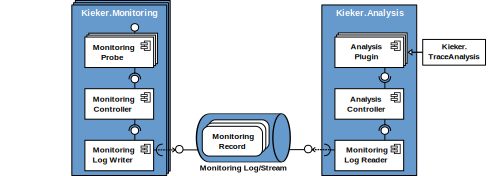
\includegraphics[width=0.81\textwidth]{images/kiekerComponentDiagram-woCloud-bw-w-record-newNames-withTraceAnalysis-colors}
			
			\caption{Overview of the framework components}
			\label{fig:KiekerComponentDiagram}
		\end{figure}
	
	\section{Download and Installation}
		
		The \Kieker{} download site\footnote{\KiekerDownloadURL{}} provides archives of the binary and source distribution, the Javadoc~API, as well as additional examples. The Java sources presented in this user guide, as well as pre-compiled binaries, are included in the \file{\exampleDir/} directory. The file \file{\mainJar{}} contains the \KiekerMonitoringPart{} and \KiekerAnalysisPart{} components, as well as the \KiekerTraceAnalysis{} tool. In addition to the \file{\mainJar{}} file, the \file{dist/} directory includes variants of this \file{.jar} files with integrated third-party libraries. Additional information on these \file{.jar} files and when to use them will follow later in this document.
		
	\section{Licensing}
		\Kieker{} is licensed under the Apache License, Version 2.0. You may obtain a copy of the license at \url{http://www.apache.org/licenses/LICENSE-2.0}. The \Kieker{} source and binary release archives include a number of third-party libraries. The \dir{lib/} directory of the release archives contains a \file{.LICENSE} file for each third-party library, pointing to the respective license text.	
		
	\section{Citing Kieker}\label{sec:ch1:citingKieker}
		When referencing Kieker resources in your publications, we would be happy if you respected the following guide lines:

		\begin{itemize}
			\item 
			When referencing the Kieker project, please cite our ICPE~2012~\cite{KiekerICPE2012} paper and/or our 2009 technical report~\cite{vanHoornRohrHasselbringWallerEhlersFreyKieselhorst2009TRContinuousMonitoringOfSoftwareServicesDesignAndApplicationOfTheKiekerFramework}. Also, you might want to add a reference to our web site (\url{http://kieker-monitoring.net/}) like~\cite{KiekerWebSite}. 
			\item 
			When referencing this user guide, e.g., when reprinting contents, please use a citation like~\cite{Kieker1.7UserGuide}.
		\end{itemize}

		\noindent At \url{http://kieker-monitoring.net/research/publications/} we provide entries for $\mathrm{B\scriptstyle IB}\!$\TeX{} and other bibliography systems.
		
	\section{Outline of this User Guide}
		The rest of this user guide is structured as followed. Chapter~\ref{chp:Quickstart-Example} contains a short quickstart example. In Chapter~\ref{chp:Kieker-Monitoring} we provide a detailed description of \KiekerMonitoringPart{} and its components, before presenting in Chapter~\ref{chp:Kieker-Analysis} the \KiekerAnalysisPart{} and its important parts. Various tools, which \Kieker{} already provides, can be found in Chapter~\ref{chp:Kieker-Tools}. The \hyperlink{hypertarget:appendix}{Appendix} finally includes additional resources, e.g., how to use the JMS writers and readers.
  \chapter{Quick Start Example}

This chapter provides a brief introduction to \Kieker{} based on a simple Bookstore example application. %
Section \ref{sec:example:downloadInstall} explains how to download and install \Kieker{}. The Bookstore application itself is introduced in Section \ref{sec:example:bookstore}, while the following Sections \ref{sec:example:monitoring} and \ref{sec:example:analysis} demonstrate how to use \Kieker{} for monitoring and analyzing the resulting monitoring data.

\section{Download and Installation}\label{sec:example:downloadInstall}

\Kieker{} can be downloaded from \KiekerURL. The web site provides zip/tar.gz archives of the \Kieker{} binary distribution as well as the corresponding \Kieker{} source code archives.

For this chapter, it is required to download and extract an archive containing \Kieker's binary distribution, e.g., \file{\binaryFileForDownload}. The extracted content has roughly the following directory structure:
% Note: The indention is not really necessary, but the tree is easier to understand in the tex-source.
\begin{figure}[H]
\begin{graybox}
\dirtree{%  
	.1 \DirInDirTree{\KiekerDir/}.
		.2 \DirInDirTree{bin/}\DTcomment{Call scripts for \Kieker{} tools}. 
			.3 \ldots. 
		.2 \DirInDirTree{doc/}\DTcomment{}. 
			.3 \DirInDirTree{tutorial/}. 
				.4 userguide.pdf\DTcomment{PDF file of this document}. 
				.4 source-example/\DTcomment{Source code of the examples in this document}. 
		.2 \DirInDirTree{dist/}\DTcomment{The \Kieker{} framework libraries}. 
			.3 \analysisJar. 
			.3 \commonJar. 
			.3 \monitoringJar. 
			.3 \toolsJar. 
		.2 \DirInDirTree{lib/}\DTcomment{Libraries required by \Kieker{}}. 
			.3 \ldots. 
		.2 \DirInDirTree{META-INF/}\DTcomment{Example configuration files}. 
			.3 \ldots. 
}
\end{graybox}
\caption{Directory structure and contents of \Kieker{}'s binary distribution}
\end{figure}

\section{Bookstore Example Application}\label{sec:example:bookstore}

The Bookstore application is a small sample application resembling a simple %
bookstore where a user can search for books in an online catalog. %
Figure~\ref{fig:bookstore:classAndSequenceDiagrams} \ldots

\begin{figure}[h]\centering
\subfigure[]{\label{fig:boostore:classdiagram}%
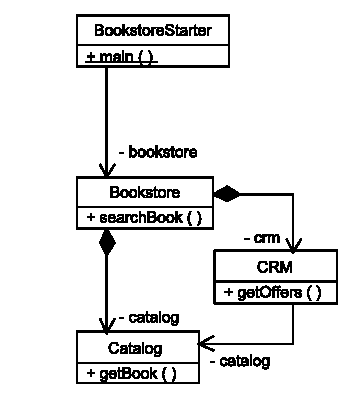
\includegraphics[scale=0.8]{images/kieker_bookstoreclassdiagram}%
}%
\subfigure[]{\label{fig:boostore:sequencediagram}%
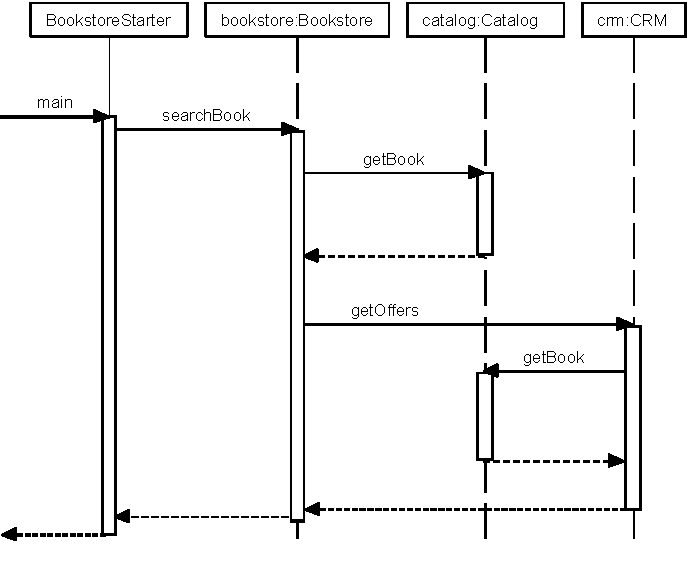
\includegraphics[scale=0.8]{images/kieker_SequenceDiagram-manually-changed}%
}
\caption{UML class diagram~\subref{fig:boostore:classdiagram} and %
sequence diagram~\subref{fig:boostore:classdiagram} of the Bookstore application}
\label{fig:bookstore:classAndSequenceDiagrams}
\end{figure}


\noindent Figure~\ref{Figure:PlainBookstoreExample} shows the directory structure of the application.

\begin{figure}[H]
\begin{graybox}
\dirtree{%
.1 \DirInDirTree{example/}. %\DTcomment{The root directory of the project}.
.2 \DirInDirTree{build/}\DTcomment{Directory for the Java class files}. 
.2 \DirInDirTree{src/}\DTcomment{The directory for the source code files}.
.3 \DirInDirTree{bookstoreApplication/}.
.4 Bookstore.java.
.4 BookstoreStarter.java.
.4 Catalog.java.
.4 CRM.java.  
}
\end{graybox}

\caption{The directory structure of the Bookstore application}
\label{Figure:PlainBookstoreExample}
\end{figure}

\noindent The following listings show the content of the source code files:

\setJavaCodeListing
\lstinputlisting[caption=Bookstore.java]{source-example/plain-example/src/bookstoreApplication/Bookstore.java}
\lstinputlisting[caption=CRM.java]{source-example/plain-example/src/bookstoreApplication/CRM.java}
\lstinputlisting[caption=Catalog.java]{source-example/plain-example/src/bookstoreApplication/Catalog.java}
\lstinputlisting[caption=BookstoreStarter.java]{source-example/plain-example/src/bookstoreApplication/BookstoreStarter.java}

\noindent The example can be compiled and executed as follows:
\setBashListing
% \begin{lstlisting}
nils@Laptop:~/example/$ javac src/mySimpleKiekerExampleManual/*.java -d build

nils@Laptop:~/example/$ java -classpath ./build/:./lib/commons-logging-1.1.1.jar\
                        mySimpleKiekerExampleManual.BookstoreMonitoringStarter 
\end{lstlisting}
% \WARNBOX{The default command-line interpreter of Windows doesn't support automatic file expansion. Therefore every single sourcefile has to be passed:
\begin{lstlisting}[caption=Commands to compile and run the Bookstore application]
#\lstshellprompt{}# javac src/bookstoreApplication/Bookstore.java 
        src/bookstoreApplication/BookstoreStarter.java 
        src/bookstoreApplication/Catalog.java 
        src/bookstoreApplication/CRM.java 
        -d build/

#\lstshellprompt{}# java -classpath build/ bookstoreApplication.BookstoreStarter 
\end{lstlisting}
%
%}

\noindent The following listing shows an example run of the application:
\begin{lstlisting}[caption=Example run of the ``plain'' application,label=lst:result-noinstr]
Bookstore.main: Starting request 0
Bookstore.main: Starting request 1
Bookstore.main: Starting request 2
Bookstore.main: Starting request 3
Bookstore.main: Starting request 4
\end{lstlisting}


\section{Monitoring}\label{sec:example:monitoring}
For the monitoring it is necessary to add some libraries from the \Kieker{}-framework to the example directory:
\begin{figure}[H]
\begin{graybox}
\dirtree{%
.1 \DirInDirTree{example/}. %\DTcomment{The root directory of the project}.
.2 \DirInDirTree{build/}\DTcomment{Directory for the Java class files}. 
.2 \newFileDirInDirTree{\DirInDirTree{lib/}}\DTcomment{Directory for the required libraries}.
.3 \newFileDirInDirTree{\monitoringJar}.
.3 \newFileDirInDirTree{\commonJar}.
.3 \newFileDirInDirTree{\commonsLoggingJar}.
.2 \DirInDirTree{src/}\DTcomment{The directory for the source code files}.
.3 \ldots.
}
\end{graybox}
\end{figure}

\noindent The \Kieker{} jar-files must be copied from the \dir{\KiekerDir/dist/} directory %
of the \Kieker{} release, as described in Section~\ref{sec:example:downloadInstall}. %
The file \file{commons-logging-1.1.1.jar} is included in \dir{\KiekerDir/lib/} %
and can also be copied from there.

The monitoring itself is done manually. Although this is not the strength of \Kieker\ it is pretty good for a quick start. Following listing shows how a method call is monitored:
\TODO{Imports?!\\ --- avh: ja, evtl. mit linerange, aber er bl\"oderweise nummeriert er so durch}
% Make sure that this listing will be modified, once the sourcecode changes!!!
% It must show the whole monitoring of the bookstorecall, from getting the first time to persisting of the record!!
\setJavaCodeListing
\lstinputlisting[linerange={11-29}, firstnumber=11, caption=Instrumentation of the \method{getBook()} call in Bookstore.java, label=listing:cuttingBookstore]%
{source-example/manual-monitoring/src/bookstoreApplication/Bookstore.java}
 
\noindent The time before and after a specific method call (in this case: \method{searchBook()}) is remembered. These information are stored in the so called operation execution record. Its (partially) layout can be seen in Figure \ref{Figure:OperationExecutionRecordClassDiagram}.

\begin{figure}[H]
\begin{centering}
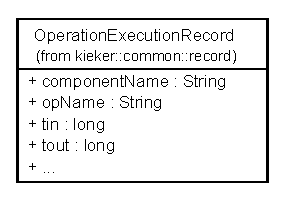
\includegraphics[scale=1]{images/kieker_OperationExecutionRecord-notraceattributes}%
\caption{The class diagram of the operation execution record}
\label{Figure:OperationExecutionRecordClassDiagram}
\end{centering}
\end{figure}

\noindent The important attributes for now are:
\begin{compactitem}
\item \class{componentName:} The component (the class) in which the called method is.
\item \class{opName:} The called method.
% \item traceId: The trace id of the current trace we want to record. Due to the fact, that we follow only one trace, this is zero in all recordings.
\item \class{tin:} The time before the source code which should be measured.
\item \class{tout:} The time after the source code which should be measured.
\end{compactitem}

\quad\\

\noindent As an example, another method in \file{CRM.java} is monitored as well:

\setJavaCodeListing
\lstinputlisting[firstline=16, firstnumber=16, lastline=27, caption=Instrumentation of the \method{getBook()} call in CRM.java, label=listing:cuttingCRM]%
{source-example/manual-monitoring/src/bookstoreApplication/CRM.java}
The instrumented example can now be compiled and executed as follows:

\setBashListing 		
\begin{lstlisting}
nils@Laptop:~/example$ javac src/mySimpleKiekerExampleManual/*.java\
 -classpath ./lib/°\commonJar°:./lib/°\monitoringJar°:\
 -d build

nils@Laptop:~/example$ java\
-classpath ./build/:\
./lib/°\commonJar°:./lib/°\monitoringJar°:./lib/°\commonsLoggingJar°\
mySimpleKiekerExampleManual.BookstoreMonitoringStarter 
\end{lstlisting}
	

\begin{lstlisting}[caption=Commands to compile and run the instrumented Bookstore under Windows,label=lst:bookstoreStarterWin]
#\lstshellprompt{}# mkdir build
#\lstshellprompt{}# javac src\bookstoreApplication\*.java -classpath lib\#\mainJar# -d build\

#\lstshellprompt{}# java -classpath build\;
       lib\#\mainJar#;
       lib\#\commonsLoggingJar#
       bookstoreApplication.BookstoreStarter 
\end{lstlisting}


\WARNBOX{%
The default command-line interpreter of Windows doesn't support automatic %
file expansion. Therefore every single source file has to be passed, as %
shown in Listing~\ref{lst:bookstoreStarterWin}. %
Also, it is necessary to separate the different elements of the classpath with %
a semicolon instead of a colon.}

\noindent If everything worked correctly, there should now be a new directory with the %
name \dir{tpmon-20100727-181422131-UTC/} (just with another timestamp) in the default %
temporary directory (under Linux this should be \dir{/tmp/}; under Windows %
\dir{C:\textbackslash{}temp\textbackslash{}}). In this directory, there should be a file with the extension %
\dir{.dat} which contains the recorded information from the source code and %
a file named \dir{tpmon.map} which contains information about the types of the %
monitoring records. %
The Listings~\ref{listing:exampledat} and \ref{listing:examplemap} show example %
contents. 
\begin{figure}[H]
\begin{graybox}
\dirtree{%
.1 \DirInDirTree{/tmp/}.
.2 \DirInDirTree{tpmon-20100727-181422131-UTC/}.
.3 tpmon.map.
.3 tpmon-20100727-181422234-UTC-Thread-2.dat.
}
\end{graybox}
\end{figure}

\setBashListing
\lstinputlisting[caption=tpmon-20100727-181422234-UTC-Thread-2.dat (excerpt), firstline=1, lastline=3, label=listing:exampledat]%
{ch2-quickstart-example/tpmon-20100727-181422131-UTC/tpmon-20100727-181422234-UTC-Thread-2.dat}

\lstinputlisting[caption=tpmon.map, label=listing:examplemap]%
{ch2-quickstart-example/tpmon-20100727-181422131-UTC/tpmon.map}

\noindent The \file{.dat}-file is saved as a CSV-file (\textbf{C}omma \textbf{S}eparated \textbf{V}alues), meaning that it can be opened with Microsoft Excel or OpenOffice.org Calc. It would be possible to visualize the stored data with the help of these programs, but we will show in Section \ref{sec:example:analysis} how to use \KiekerAnalysisPart\ to read and process the files.

\section{Analysis}\label{sec:example:analysis}
As mentioned in the beginning of this chapter, it is shown how a simple consumer is programmed before starting the analysis. Therefore we need some new files:
\begin{figure}[H]
\begin{graybox}
\dirtree{%  
.1 \DirInDirTree{example/}. 
.2 \DirInDirTree{build/}\DTcomment{Directory for the Java class files}. 
.2 \DirInDirTree{lib/}\DTcomment{Directory for the required libraries}.
.3 \ldots. 
.3 \newFileDirInDirTree{\analysisJar}.
.2 \DirInDirTree{src/}\DTcomment{The directory for the source code files}.
.3 \DirInDirTree{bookstoreApplication/}.
.4 \ldots. 
.4 \newFileDirInDirTree{BookstoreAnalysisStarter.java}.
.4 \newFileDirInDirTree{Consumer.java}.
}
\end{graybox}
\end{figure}

\noindent The new jar-file can again be found in \dir{\KiekerDir/dist}. Listing \ref{listing:Consumer} shows the content of the new created \dir{Consumer.java}. It implements the \class{IMonitoringRecordConsumerPlugin} and overrides the necessary methods so that it can later be used by the analysis component of \Kieker. In this case the component gets a maximal response time within the constructor which will later be used to check whether a recorded method call replied fast enough or not. If the method call needed more time to response that the maximal allowed response time, it will be written directly to the error stream.\\
The methods \method{terminate} and \method{execute} don't do anything due to the fact that the consumer doesn't need any initialization. If the consumer would for example use threads then these methods would be the correct location to start and stop them.

\setJavaCodeListing       
\lstinputlisting[caption=Consumer.java, label=listing:Consumer]{source-example/manual-monitoring/src/bookstoreApplication/Consumer.java}

\noindent Now, we have to create the file \dir{BookstoreAnalysisStarter.java} to analyze our recorded information. 

The analysis consists thereby of the following steps:
\begin{compactenum}
\item Create a new instance (or more) of the class \class{AnalysisInstance}.
\item Register the plugins which should evaluate the records.
\item Register exactly one reader to read the stored information.
\item Start the analysis instance.
\end{compactenum}

\setJavaCodeListing       
\lstinputlisting[caption=BookstoreAnalysisStarter.java]{source-example/manual-monitoring/src/bookstoreApplication/BookstoreAnalysisStarter.java}
As can be seen, the application expects the output directory from the earlier monitoring run (see Section \ref{sec:example:monitoring}) as argument, which must be passed manually. Following listings show again the course of action:
\setBashListing 		
\begin{lstlisting}[caption=Commands to compile and run the analysis under \UnixLikeSystems{},label=lst:bookstoreAnalysisStarterLinux] 			
#\lstshellprompt{}# mkdir build
#\lstshellprompt{}# javac src/kieker/examples/userguide/ch2bookstore/manual/*.java 
        -classpath lib/#\mainJarEMF# -d build/

#\lstshellprompt{}# java -classpath build/:lib/#\mainJarEMF#
       kieker.examples.userguide.ch2bookstore.manual.BookstoreAnalysisStarter 
       /tmp/kieker-20120402-163314855-UTC-myHost-KIEKER-SINGLETON
\end{lstlisting}		
\begin{lstlisting}[caption=Commands to compile and run the analysis under Windows,label=lst:bookstoreAnalysisStarterWin]
#\lstshellprompt{}# mkdir build
#\lstshellprompt{}# javac src\kieker\examples\userguide\ch2bookstore\manual\*.java 
        -classpath lib\#\mainJarEMF# -d build\

#\lstshellprompt{}# java -classpath build\;lib\#\mainJarEMF#
       kieker.examples.userguide.ch2bookstore.manual.BookstoreAnalysisStarter 
       C:\Temp\kieker-20130910-120352847-UTC-myHost-KIEKER-SINGLETON
\end{lstlisting}	

	
It should be ensured that the application gets the correct path from the monitoring run. 

If everything worked correctly, the consumer should write something on the outputstream for every record it gets. A possible display of the run can be found in the appendix of this tutorial. 
  %%%%%%%%%%%%%%%%%%%%%%%%%%%%%%%%%%%%%%%%%
% Kieker Monitoring Component
% 
% $Date$
% $Rev$:
% $Author$


\chapter{\KiekerMonitoringPart{} Component}\label{chap:componentsMonitoring}

\NOTIFYBOX{The Java sources of this chapter can be found in the %
\file{\customComponentsBookstoreApplicationDirDistro{}/} directory of the %
binary release.}

\section{Monitoring Controller}\label{sec:componentsMonitoring:monitoringController}

The \class{MonitoringController} constructs and controls a \KiekerMonitoringPart{} %
instance. As depicted by the class diagram in Figure~\ref{fig:monitoringController:classdiagram}, it provides methods for\\

\enlargethispage{1cm}

\begin{figure}\centering % [H]
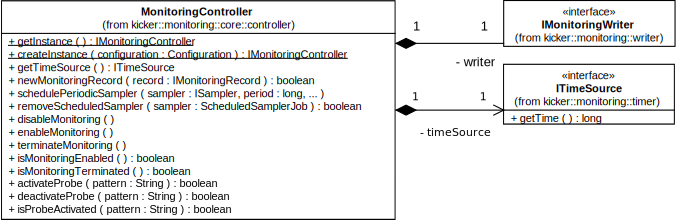
\includegraphics[scale=0.7]{images/kieker_monitoringControlleruserguide-simplified}
\caption{Class diagram of the \class{MonitoringController} (including selected methods)}
\label{fig:monitoringController:classdiagram}
\end{figure}

\begin{compactitem}
 \item Creating \class{IMonitoringController} instances (Section~\ref{sec:componentsMonitoring:monitoringController:factory}),
 \item Logging monitoring records employing the configured monitoring writer (Section~\ref{sec:componentsMonitoring:monitoringController:logging}), 
 \item Retrieving the current time via the configured time source (Section~\ref{sec:componentsMonitoring:monitoringController:getTime}),
 \item Scheduling and removing period samplers (Section~\ref{sec:componentsMonitoring:monitoringController:periodicSamplers}), and
 \item Controlling the monitoring state (Section~\ref{sec:componentsMonitoring:monitoringController:controState}).
\end{compactitem}

\subsection{Creating \class{MonitoringController} Instances}\label{sec:componentsMonitoring:monitoringController:factory}

The \class{MonitoringController} provides two different static methods for retrieving instances of %
\class{IMonitoringController}:\\

\begin{compactenum}
 \item The method \method{MonitoringController.getInstance()} returns a singleton instance. %
As described in Section~\ref{sec:monitoring:configuration}, the configuration is read from %
a properties file that has been passed to the JVM, is located in the classpath, or %
conforms to the default configuration (Appendix~\ref{sec:appdx:monitoringproperties}). %
 \item The method \method{MonitoringController.createInstance(Configuration config)} can be used to create %
an instance that is configured according to the passed \class{Configuration} object, %
as described in Section~\ref{sec:monitoring:configuration}.
\end{compactenum}

\subsection{Logging Monitoring Records}\label{sec:componentsMonitoring:monitoringController:logging}

Monitoring records are sent to the configured monitoring writers by passing %
these records, in form of \class{IMonitoringRecord} objects, to the %
\class{MonitoringController}'s \method{newMonitoringRecord} method.  %
Note, that this is not the case if monitoring is disabled or terminated (Section~\ref{sec:componentsMonitoring:monitoringController:controState}). 

\subsection{Retrieving the Current Time and Using Custom Time Sources}\label{sec:componentsMonitoring:monitoringController:getTime}

The current time is maintained by a so-called time source. The \class{MonitoringController}'s method %
\method{getTimeSource} returns an \class{ITimeSource} object which provides a method %
\method{getTime}. \Kieker{}'s default time source (\class{DefaultSystemTimer}) returns the current system %
time as the number of nanoseconds elapsed since 1 Jan 1970 00:00~UTC. %
The easiest way to use a custom time source is to extend the \class{AbstractTimeSource} and %
to implement the method \method{getTime()}. Custom time sources make sense, for example, %
in simulations where not the current system time but the current simulation time is %
relevant. The configuration needs to be adjusted to use a custom time source class. %

\subsection{Scheduling and Removing Periodic Samplers}\label{sec:componentsMonitoring:monitoringController:periodicSamplers}

For certain applications, it is required to monitor runtime data periodically, %
e.g., the utilization of system resources such as CPUs. %
For this purpose, \Kieker{} supports special monitoring probes, called samplers. %
Samplers must implement the interface \class{ISampler} which includes a %
single method \method{sample(IMonitoringController monitoringController)}. %
This method is called in peridioc time steps, %
as specified by the \class{MonitoringController}'s registration function %
\method{schedulePeriodicSampler}. Periodic samplers can be stopped by %
calling the \class{MonitoringController}'s method \method{removeScheduledSampler}.

Listing~\ref{listing:sigarSamplerMethod} shows the \method{sample} method %
of the \class{MemSwapUsageSampler} which can be used to monitor memory %
and swap usage employing the Sigar library~\cite{HypericSigarWebsite}. %
Likewise to other monitoring probes described in this user guide (see for %
example Sections~\ref{sec:monitoring:probe} and \ref{sec:example:monitoring}), 
it collects the data of interest (lines~57--58), creates a monitoring record~%
(lines~59--64), and passes this monitoring record to the monitoring controller~%
(line~65). %
The available Sigar-based samplers for monitoring system-level monitoring %
data, such as CPU and memory usage, are discussed in Appendix~\ref{appendix:SigarBasedSamplers}. %

\pagebreak

\setJavaCodeListing
\lstinputlisting[firstline=55, lastline=66, firstnumber=55, caption=Method \method{sample} from MemSwapUsageSampler.java, label=listing:sigarSamplerMethod]{\kiekerSrcDir/monitoring/kieker/monitoring/probe/sigar/samplers/MemSwapUsageSampler.java}

\subsection{Controlling the Monitoring State}\label{sec:componentsMonitoring:monitoringController:controState}

The \class{MonitoringController} provides methods to temporarily enable or disable monitoring %
(\method{enableMonitoring}/\method{disableMonitoring}), as well as to terminate monitoring %
permanently (\method{terminateMonitoring}). %
The current state can be requested by calling the methods \method{isMonitoringEnabled} %
and \method{isMonitoringTerminated}. If monitoring is not enabled (i.e., disabled %
or terminated), no monitoring records retrieved via the method \method{newMonitoringRecord} %
are passed to the monitoring writer. Also, probes should be passive or return immediately %
with respect to the return value of the method \method{isMonitoringEnabled}. %
Note, that once the \class{MonitoringController} is terminated, it cannot be enabled %
later on. 

\subsection{JMX MBean Access to \class{MonitoringController}}

\begin{figure}\centering
\subfigure[Attributes]{%
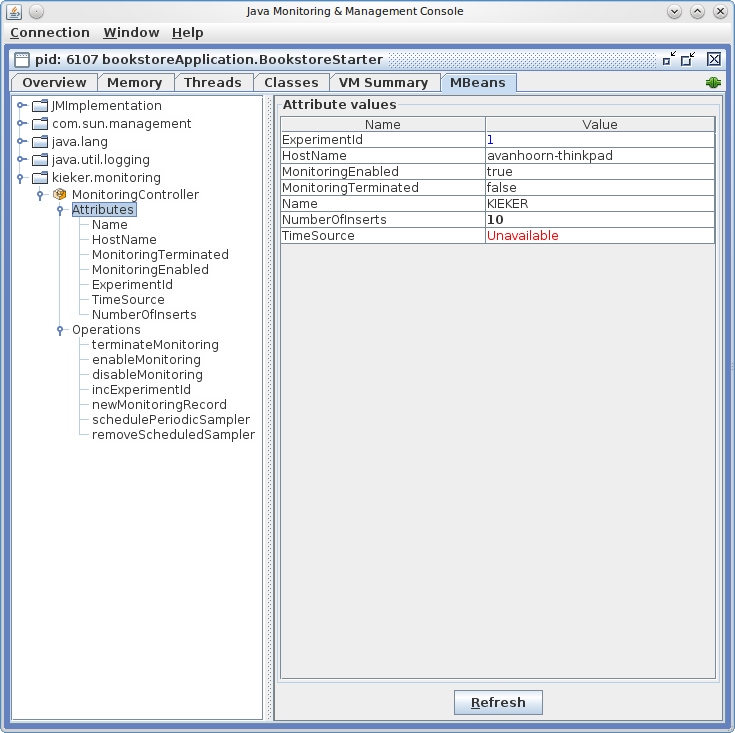
\includegraphics[width=0.485\textwidth]{images/jmxbean-monitoringcontroller-attributes.png}
}
\subfigure[Operations]{%
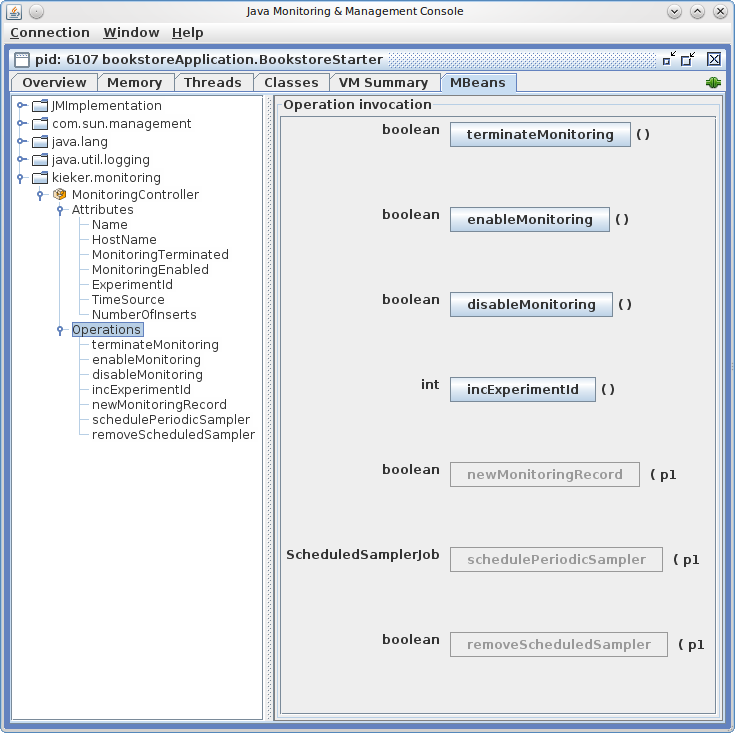
\includegraphics[width=0.485\textwidth]{images/jmxbean-monitoringcontroller-operations.png}
}  
\caption{Screenshots of the \class{jconsole} JMX client accessing the \class{MonitoringController}'s %
attributes and operations via the MBean interface. %
}
\label{fig:monitoringController:MBean:jconsole}
\end{figure}

The \class{MonitoringController}'s %
interface methods (see Figure~\ref{fig:monitoringController:classdiagram}) can be accessed %
as a JMX MBean. For example, this allows to control the monitoring state using %
the methods described in the previous Section~\ref{sec:componentsMonitoring:monitoringController:controState}. %
As a JMX-compliant graphical client that is included in the JDK, \class{jconsole} %
is probably the easiest way to get started. Figure~\ref{fig:monitoringController:MBean:jconsole} %
shows two screenshots of the MBean access using \class{jconsole}.

In order to enable JMX MBean access to the \class{MonitoringController}, the value of the %
configuration property \textit{kieker.monitoring.MBean} must be set to \textit{true}:\\

\setPropertiesListing
\begin{lstlisting}
 # Whether the MonitoringController will be available as an MBean.
kieker.monitoring.MBean=true
\end{lstlisting}

\section{\KiekerMonitoringPart{} Configuration}\label{sec:monitoring:configuration}

\KiekerMonitoringPart{} instances can be configured by properties files, %
\class{Configuration} objects, and by passing property values as %
JVM arguments. If no configuration is specified, a default %
configuration is being used. %
Appendix~\ref{sec:appdx:monitoringproperties} lists this default %
configuration with a documentation of all available properties. %
The default configuration properties file, which %
can be used as a template for custom configurations, is provided by the file %
\file{\monitoringPropertiesFile} in the directory \dir{\KiekerDir/META-INF/} of %
the binary release (see Section~\ref{sec:example:downloadInstall}). %


\subsection*{Configurations for Singleton Instances}

In order to use a custom configuration file, its location needs to be passed to %
the JVM using the parameter \textit{kieker.monitoring.configuration} as follows:

\setBashListing
\begin{lstlisting}[caption=,label=lst:monitoringPropertiesPassedToJVM]
#\lstshellprompt# java	#\textbf{-Dkieker.monitoring.configuration=}#<ANY-DIR>/my.kieker.monitoring.properties #[\ldots]#
\end{lstlisting}

\noindent Alternatively, a file named \file{kieker.monitoring.properties} %
can be placed in a directory called \dir{META-INF/} located in the classpath. %
The available configuration properties can also be passed as JVM %
arguments, e.g., \lstinline{-Dkieker.monitoring.enabled=true}. %

\subsection*{Configurations for Non-Singleton Instances}

The class \class{Configuration} provides factory methods to create %
\class{Configuration} objects according to the default configuration %
or loaded from a specified properties file: \method{createDefaultConfiguration}, %
\method{createConfigurationFromFile}, and \method{createSingletonConfiguration}. %
Note, that JVM parameters are only evaluated when using the factory method %
\method{createSingletonConfiguration}. %
The returned \class{Configuration} objects can be adjusted by setting %
single property values using the method \method{setProperty}. %

\section{Monitoring Records}\label{sec:componentsMonitoring:monitoringRecords}

Monitoring records are objects that contain the monitoring data, as mentioned %
in the previous chapters. Typically, an instance of a monitoring record is %
constructed in a monitoring probe (Section~\ref{sec:monitoring:probe}), %
passed to the monitoring controller (Section~\ref{sec:componentsMonitoring:monitoringController}), %
serialized and deserialized by a monitoring %
writer (Section~\ref{sec:monitoring-log-writers}) and a
monitoring reader (Section~\ref{sec:analysis:reader}), and provided to the %
analyis plugins (Section~\ref{sec:analysis:consumer}) %
by the analysis controller (Section~\ref{sec:analysis:controller}). %
Figure~\ref{fig:KiekerCommunicationDiagram} illustrates this life cycle of a monitoring %
record. %

In Chapter~\ref{chap:example}, we've already introduced and used the monitoring %
record type \class{OperationExecutionRecord}. \Kieker{} allows to use custom %
monitoring record types. Corresponding classes must implement the %
interface \class{IMonitoringRecord} shown in Figure~\ref{sec:monitoringrecord:interfacesAndImplementingClasses}. %
The methods \method{initFromArray}, \method{toArray}, \method{getValueTypes} %
are used for serialization and deserialization of the monitoring data contained %
in the record. The method \method{setLoggingTimestamp} is used by the monitoring controller to %
store the date and time when a record is received by the controller. %
The method \method{getLoggingTimestamp} can be used during analysis to retrieve %
this value. \KiekerMonitoringPart{} provides the abstract class %
\class{AbstractMonitoringRecord} (Figure~\ref{sec:monitoringrecord:interfacesAndImplementingClasses}) %
which already implements the methods to maintain the logging timestamp. 

\begin{figure}[h]\centering
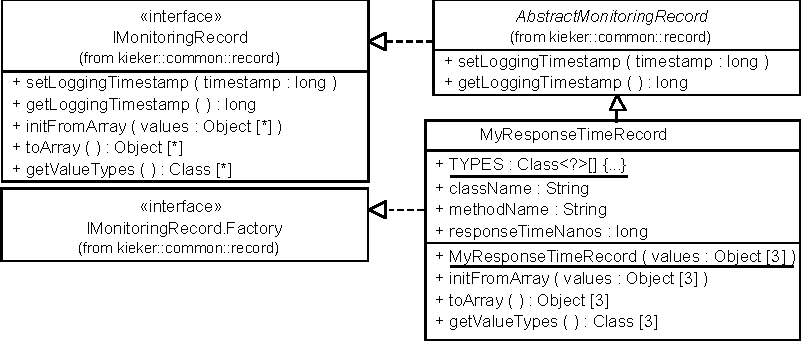
\includegraphics[scale=0.7]{images/kieker_MyRTRecord-modified}
\caption{Class diagram with the \class{IMonitoringRecord} interface, the abstract %
class \class{AbstractMonitoringRecord}, and a custom monitoring record type %
\class{MyResponseTimeRecord}}
\label{sec:monitoringrecord:interfacesAndImplementingClasses}
\end{figure}

\pagebreak

\noindent In order to use the abstract class for implementing your own monitoring record type, you need to:

\begin{enumerate}
\item Create a class that extends \class{AbstractMonitoringRecord}  and
\item Override the methods \method{initFromArray}, \method{toArray}, \method{getValueTypes}.
\end{enumerate}

\noindent The class \class{MyResponseTimeRecord}, shown in the class diagram in %
Figure~\ref{sec:monitoringrecord:interfacesAndImplementingClasses} and in %
Listing~\ref{listing:MyRecord}, is an example of a custom monitoring record type %
that can be used to monitor response times of method executions.

\setJavaCodeListing
\lstinputlisting[caption=MyResponseTimeRecord.java, label=listing:MyRecord,firstline=21,firstnumber=21]{\customComponentsBookstoreApplicationDir/src/bookstoreApplication/MyResponseTimeRecord.java}

\pagebreak

\section{Monitoring Probes}\label{sec:monitoring:probe}

The probes are responsible for collecting the monitoring data and passing it %
to the monitoring controller. %
In Chapter~\ref{sec:example:monitoring}, we have already demonstrated how to %
manually instrument a Java application. Listing~\ref{listing:cuttingBookstore} %
shows a similar manual monitoring probe which uses the monitoring record type %
\class{MyResponseTimeRecord} defined in the previous Section~\ref{sec:componentsMonitoring:monitoringRecords}.

% Make sure that this listing will be modified, once the sourcecode changes!!!
% It must show the whole monitoring of the bookstorecall, from getting the first time to persisting of the record!!
\lstinputlisting[firstline=35, lastline=46, firstnumber=35, caption=Excerpt from Bookstore.java, label=listing:cuttingBookstore]{\customComponentsBookstoreApplicationDir/src/bookstoreApplication/Bookstore.java}

\noindent In order to avoid multiple calls to the \method{getInstance} method of the %
\class{MonitoringController} class, singleton instances should be stored %
in a final static variable, as shown in Listing~\ref{listing:cuttingBookstore:finalStaticController}.

\lstinputlisting[firstline=30, lastline=31, firstnumber=30, caption=Singleton instance of the monitoring controller stored in a final static variable (excerpt from Bookstore.java), label=listing:cuttingBookstore:finalStaticController]{\customComponentsBookstoreApplicationDir/src/bookstoreApplication/Bookstore.java}

\noindent When manually instrumenting an application, the monitoring probe is implemented %
by mixing monitoring logic with business logic, which is often not desired since %
the resulting code is hardly maintainable. %
Many middleware technologies, such as Java~EE Servlet~\cite{JavaServletTechnology-WebSite}, %
Spring~\cite{Spring-WebSite}, and %
Apache~CXF~\cite{CXF-WebSite} provide interception/AOP~\cite{Kiczales1997} interfaces %
which are well-suited to implement monitoring probes. AspectJ~\cite{AspectJ-WebSite} allows to %
instrument Java applications without source code modifications. %
Chapter~\ref{chap:aspectJ} describes the \Kieker{} probes based on these technologies allowing to %
monitor trace information in distributed applications. 

\section{Monitoring Writers}\label{sec:monitoring-log-writers}

Monitoring log writers serialize monitoring records to the monitoring log and  % and persist the recorded informations into files, databases etc. %
must implement the interface \class{IMonitoringWriter}. The monitoring %
controller passes the received records to the writer by calling the method %
\method{newMonitoringRecord}. Writers can use the methods to serialize the %
record contents, as described in Section~\ref{sec:componentsMonitoring:monitoringRecords}. 

Figure~\ref{figure:monitoringLogWritersHierarchy} shows the monitoring writers %
already implemented in \KiekerMonitoringPart{}. The writers \class{AsyncFsWriter}, %
\class{SyncFsWriter}, \class{AsyncDbWriter}, and \class{SyncDbWriter} can be used %
to store monitoring records to filesystems and databases respectively. %
The variants with the prefix \class{Async} are implemented using asynchronous %
threads that decouple the I/O operations from the control flow of the %
instrumented application. % 
The \class{AsyncFsWriter} is the default writer which has already been used in %
Section~\ref{sec:example:monitoring}. %
Currently, the database writer only supports the record type \class{OperationExecutionRecord}. %

The \class{AsyncJMSWriter} writes records to a JMS (Java Messaging Service~\cite{JMS-WebSite}) queue. %
This allows to implement on-the-fly analysis in distributed systems, i.e., analysis while %
continuously receiving new monitoring data from an instrumented application potentially %
running on another machine. A brief description of how to use the \class{AsyncJMSWriter} %
can be found in Appendix~\ref{appendix:usingJMS}. %

% This is the diagram with the hierarchy of the writers.
\begin{figure}[H]
\begin{centering}
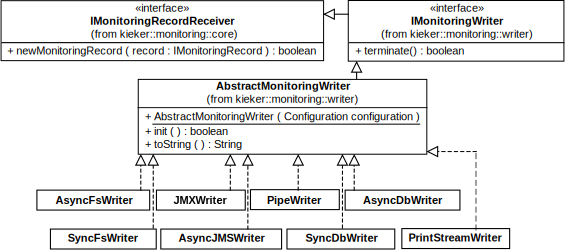
\includegraphics[scale=0.7]{images/kieker_writerimplsuserguide-modified}
\caption{Interface \class{IMonitoringLogWriter} and  the implementing classes}
\label{figure:monitoringLogWritersHierarchy}
\end{centering}
\end{figure}

\noindent Listing~\ref{listing:MyWriter} on page~\pageref{listing:MyWriter} shows %
a custom writer \class{MyPipeWriter} which uses a named pipe to %
write the given records into a buffer located in the memory. The source code of %
the class \class{MyPipe} is listed in Appendix~\ref{appendix:pipeListings}. %

\setJavaCodeListing
\lstinputlisting[caption=MyWriter.java, label=listing:MyWriter,float,firstline=21,firstnumber=21]{\customComponentsBookstoreApplicationDir/src/bookstoreApplication/MyPipeWriter.java}

\noindent The monitoring writer to be used is selected and configured by the \KiekerMonitoringPart{} %
configuration properties (Section~\ref{chap:componentsMonitoring}) %
\textit{monitoringDataWriter} and \textit{monitoringDataWriterInitString}. %
Listing~\ref{lst:monitoringwriter:MyWriter} demonstrates how to use the custom %
writer \class{MyPipeWriter} defined above. In this example, the pipe name is %
passed as the property value \textit{monitoringDataWriterInitString}.

\setBashListing       
\begin{lstlisting}[label=lst:monitoringwriter:MyWriter]
monitoringDataWriter=bookstoreApplication.MyPipeWriter
monitoringDataWriterInitString=pipeName=somePipe
\end{lstlisting}

\enlargethispage{1cm}

\noindent As the data structure for this kind of monitoring log, we created a %
class \class{PipeData} in order to demonstrate the use of the \method{toArray} and %
\method{initFromArray} (in Section~\ref{sec:analysis:reader}) methods. %
A \class{PipeData} object holds a logging timestamp and an \class{Object} array %
containing the serialized record data. % 
Appendix~\ref{appendix:pipeListings} includes a source code listing of this class. %
Alternatively, we could have used \class{IMonitoringRecord} as the data structure %
used by the pipe. This is the way, \Kieker{}'s \class{PipeWriter} works. %

  %%%%%%%%%%%%%%%%%%%%%%%%%%%%%%%%%%%%%%%%%
% Kieker Analysis Component
%
% $Date$
% $Rev$:
% $Author$

\chapter{\KiekerAnalysisPart{} Component}\label{chap:componentsAnalysis}

\NOTIFYBOX{The Java sources of this chapter, as well as a pre-compiled binary, %
can be found in the %
\file{\customComponentsBookstoreApplicationDirDistro{}/} directory of the %
binary release.}

\section{Pipe-and-Filter Framework and Included Plugins}\label{sec:analysis:controller}

\KiekerAnalysisPart{} provides a framework to define and execute pipe-and-filter %
architectures of analysis plugins, i.e., monitoring readers and analysis filters, %
as well as repositories. %
This section describes how to use and develop readers, filters, and %
repositories. The description is based on the example %
pipe-and-filter architecture shown in Figure~\ref{fig:example:pipe-and-filter}. The custom monitoring reader %
\class{MyPipeReader}, which corresponds to the writer developed in Section~\ref{sec:monitoring-log-writers}, %
sends records to the connected custom filter \class{MyResponseTimeFilter}. %
This filter accepts only events of the record type \class{MyResponseTimeRecord},
developed in Section~\ref{sec:componentsMonitoring:monitoringRecords}. %
The \class{MyResponseTimeFilter} classifies incoming \class{MyResponseTimeRecord}s %
based on whether they satisfy or exceed a configured threshold and passes them %
to the respective output ports, \method{validResponseTimes} or \method{invalidResponseTimes}. %
Two instances of a second custom filter, \class{MyResponseTimeOutputPrinter}, %
print the received records to the standard output stream.

\begin{figure}
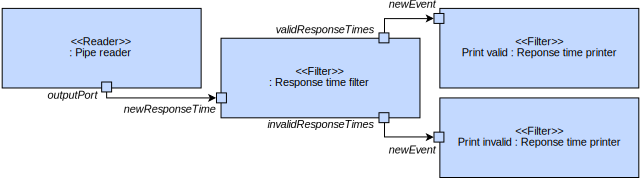
\includegraphics[width=\textwidth]{images/example-pipe-and-filter}
\caption{Example pipe-and-filter configuration}
\label{fig:example:pipe-and-filter}
\end{figure}

%  requires a monitoring reader %
% (Section~\ref{sec:analysis:reader}) and at least %
% one monitoring record consumer plugin (Section~\ref{sec:analysis:consumer}). %
% In addition to the monitoring record consumer plugin, %
% other analysis plugins can be registered. %

\begin{figure}\centering
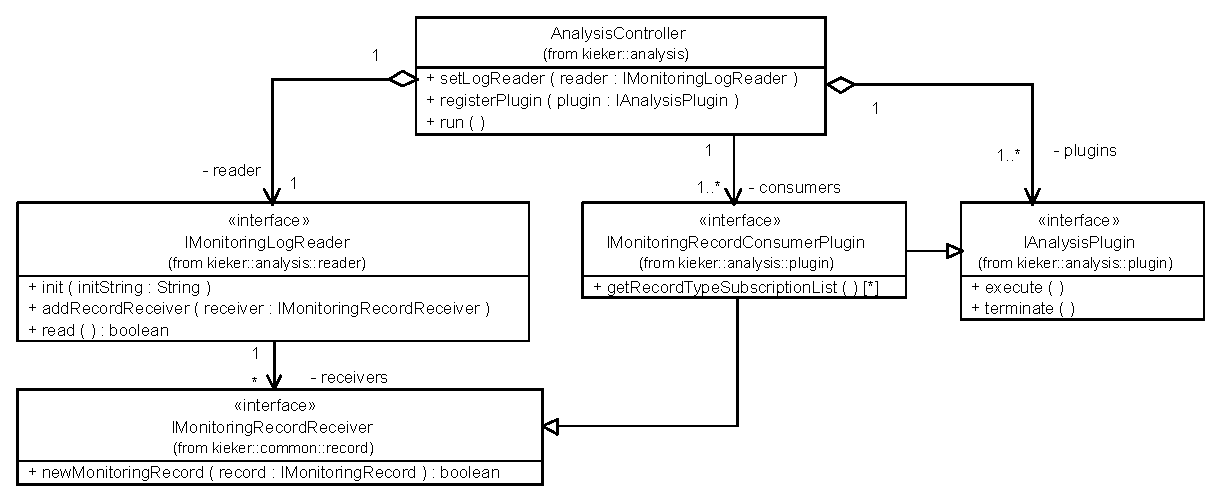
\includegraphics[width=\textwidth]{images/kieker_AnalysisControlleruserguide-modified}
\caption{Class diagram showing important \KiekerAnalysisPart{} types and their relationship}
\label{fig:analysisController:classdiagram}
\end{figure}

% \pagebreak

\noindent Figure~\ref{fig:analysisController:classdiagram} shows the class diagram %
with the important \KiekerAnalysisPart{} classes and their relationships. %
Note that only the most important methods are included. 
An analysis with \KiekerAnalysisPart{} is set up and executed employing %
the class \class{AnalysisController}. %
Setting up and running an analysis with \KiekerAnalysisPart{} requires the %
following steps to be performed, as sketched in Section~\ref{sec:example:analysis} already:

\enlargethispage{1.2cm}

\medskip

\begin{compactenum}
\item Creating an instance of the \class{AnalysisController} class
\item Creating monitoring readers, filters, and repositories.
\item Connecting plugins to other plugins and to repositories (\method{connect})
\item Starting the analysis instance (\method{run}).
\end{compactenum}

\medskip

\noindent On invocation of the \method{run} method, the \class{AnalysisController} %
calls the \method{init} method of all filter plugins allowing them to initialize. %
Then, it starts the configured monitoring readers by calling its \method{read} %
method. Plugins send data via their output ports to connected input ports of other
plugins. Being the source in a pipe-and-filter architecture, readers don't have %
input ports. Plugins can be connected to repositories, which may provide %
shared services, such as managed access to a common architectural model %
of the analyzed system. As soon as all readers have returned from the execution of their \method{read}
methods, the method \method{terminate} of each registered plugin is called by the %
\class{AnalysisController}. \KiekerAnalysisPart{} configurations can be saved %
to a \class{.kax} file by calling the \class{AnalysisController}'s \method{saveToFile} method. %
The \class{AnalysisController} provides a constructor which accepts the %
file system location of a \class{.kax} file to load the configuration from. %
See Appendix~\ref{appendix:wrapperScripts:kaxRun} and~\ref{appendix:wrapperScripts:kaxViz} %
for included tools/scripts which execute and visualize \class{.kax} files.
 %
In order to support the asynchronous execution of the \class{AnalysisController} instance, %
we provide the \class{AnalysisControllerThread} class.

\subsection{Programmatic Creation of Pipe-and-Filter Architectures}\label{sec:analysis:programmaticCreation}

To give a first impression of the programmatic %
instantiation, configuration, and connection of plugins, Listing~\ref{listing:StarterInitConnect} %
demonstrates this procedure for the example, using \class{MyPipeReader} and %
\class{MyResponseTimeFilter}, according to Figure~\ref{fig:example:pipe-and-filter}.

The configuration for the \class{MyPipeReader} is created in lines~50--51. %
Using this configuration, the reader is created in line~52. Similarly, %
lines~55--61 initialize the \class{MyResponseTimeFilter}. The reader's output is connected %
to the filter's input in line~62. %
The entire programmatic creation of the pipe-and-filter architecture shown %
in Figure~\ref{fig:example:pipe-and-filter}, can be found in the example  %
file \file{Starter.java}.

\medskip

\setJavaCodeListing
\lstinputlisting[caption=Initializing and connecting the example reader and filter (Starter.java),label=listing:StarterInitConnect,firstline=47, lastline=62, firstnumber=47]%
{\customComponentsBookstoreApplicationDir/src/kieker/examples/userguide/ch3and4bookstore/Starter.java}

\enlargethispage{0.5cm}

\subsection{Monitoring Reader Plugins}

% Warning-tag for the reader-writer-thing
The monitoring readers are the direct counterpart to the monitoring %
writers. While writers receive records and write them into files or other kinds %
of monitoring logs/streams, readers deserialize monitoring data and provide it as %
\class{IMonitoringRecord} instances.

\begin{figure}\centering
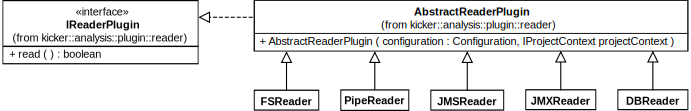
\includegraphics[scale=0.7]{images/kieker_readerimplsuserguide-modified}
\caption{Monitoring reader plugins included with \Kieker{}}
\label{Figure:ReaderHierarchy}
\end{figure}

% \pagebreak

% \
%
% \WARNBOX{This means that whenever a new writer is implemented, a corresponding reader has to be implemented as well. If one want for example to store the recorded informations in a database, one should be capable of reading these saved informations from the database again.}
%
% \

% \enlargethispage{1cm}

\noindent There are already some readers implemented in \Kieker,  as shown in the %
class diagram in Figure \ref{Figure:ReaderHierarchy}. %
The \class{FSReader} has already been used in Section~\ref{sec:example:analysis}. %
A brief description of how to use the \class{JMSReader} can be found in Appendix~%
\ref{appendix:usingJMS}. Please note that the database reader (\class{DBReader}) %
is currently in a prototype stage and that it should be used with care. %
Like each plugin, readers are configured via properties, as used in Section~%
\ref{sec:analysis:programmaticCreation} and detailed in Section~%
\ref{sec:analysis:configuration}.

\subsection{Filter Plugins}

Filter plugins receive events (Java objects) via input ports from other %
plugins and implement analyses or visualizations based on these events. %
\Kieker{} already includes some basic filter plugins. For example, the %
\class{CountingFilter} and  \class{TeeFilter} forward incoming events %
to their output ports. The \class{CountingFilter} additionally provides the %
current number of received records via a second output port. The \class{TeeFilter} %
additionally prints incoming events to an output stream, which may be %
the standard output, standard error, a logger, or a file. %
A \class{TimestampFilter} and a \class{TypeFilter} filter incoming records by %
timestamp and by type, respectively. A \class{TraceIdFilter} filters incoming %
trace events (e.g., \class{OperationExecutionRecord}s, see Section~%
\ref{chap:example}) by trace ID. Additional filters for trace analysis, %
architecture reconstruction and visualization are included as part of %
the \KiekerTraceAnalysis{} tool, presented in Chapter~\ref{chap:aspectJ}. %
Like each plugin, filters are configured %
via properties, as used in Section~\ref{sec:analysis:programmaticCreation} and %
detailed in Section~%
\ref{sec:analysis:configuration}. %

% \pagebreak
% \setJavaCodeListing
%\lstinputlisting[caption=MyReponseTimeConsumer.java,label=lst:MyReponseTimeConsumer,firstline=21,firstnumber=21]{\customComponentsBookstoreApplicationDir/src/kieker/examples/userguide/ch3and4bookstore/MyResponseTimeConsumer.java}

% The following Listing~\ref{listing:AnalysisController} shows how to create and run an analysis %
% with these custom components:
%
% \setJavaCodeListing
% \lstinputlisting[caption=Code snippet setting up and running a \KiekerAnalysisPart{} instance (Starter.java),label=listing:AnalysisController,firstline=48, lastline=82, firstnumber=48]%
% {\customComponentsBookstoreApplicationDir/src/kieker/examples/userguide/ch3and4bookstore/Starter.java}

% \enlargethispage{1.2cm}

\subsection{Repositories}

Currently, \Kieker{} includes a single repository, \class{SystemModelRepository}, %
which is used by the \KiekerTraceAnalysis{} filters to update and query %
a component-based system model representing architectural entities %
and structures discovered while processing the incoming monitoring data. %
The development and use of repositories is detailed in Section~%
\ref{sec:analysis:repositories}. %

When using components of the \KiekerTraceAnalysis{}, make sure that write access to the %
\class{SystemModelRepository} is only triggered by readers. Some filters are terminated %
after the readers and expect the repository to be in a completed state.


\section{Developing Analysis Plugins and Repositories}\label{sec:analysis:plugins}

When implementing analysis plugins (i.e., readers or filters) and repositories, %
the classes \class{AbstractReaderPlugin}, \class{AbstractFilterPlugin}, or, %
respectively, \class{AbstractRepository} need to be extended %
(Figure~\ref{fig:analysisController:classdiagram}). %
Section~\ref{sec:analysis:configuration} describes how plugins and repositories %
can be configured via properties. %
Section~\ref{sec:analysis:pluginAnnotation} %
describes how to declare meta-information for plugins using %
dedicated annotations. %
Specific information on the development of custom filters, readers, and repositories %
are given in Sections~\ref{sec:analysis:filters}--\ref{sec:analysis:repositories}. %

% The monitoring record consumer plugins described in the following %
% Section~\ref{sec:analysis:consumer}, are special analysis plugins that receive %
% the monitoring records provided by the monitoring reader. %
% Starting with these monitoring record plugins, analysis plugins can be connected %
% in a pipe-and-filter style to implement more complex analyses. %
% \Kieker{} provides input and output port interfaces and implementing classes %
% to implement such analyses. See the documentation of the classes \class{AbstractInputPort} %
% and \class{OutputPort} for details. \KiekerTraceAnalysis{} is implemented %
% based on this pattern.

\subsection{Configuration}\label{sec:analysis:configuration}

\noindent According to the %
configuration of the \KiekerMonitoringPart{} components (see Section~\ref{sec:monitoring:configuration}),
plugins and repositories are configured via \class{Configuration} objects. Classes must %
provide a public constructor, accepting a \class{Configuration} and an \class{IProjectContext} (normally the \class{IAnalysisController} instance) object as %
its only arguments. It is important to invoke the constructor of the super class. %
The configuration properties accepted by a plugin or repository should be provided via \class{public static} %
constants with prefix \method{CONFIG\_PROPERTY\_NAME\_} in order to ease the %
programmatic initialization of plugins (Section~\ref{sec:analysis:programmaticCreation}). %
For the example filter \class{MyResponseTimeFilter},
Listing~\ref{listing:MyResponseTimeFilterConstructor} shows the constructor,
the configuration property, and the corresponding member value obtained from the %
configuration.

\setJavaCodeListing
\lstinputlisting[firstline=44, firstnumber=44, lastline=52, caption={Plugin constructor accepting a \class{Configuration} and an \class{IProjectContext} object}, label=listing:MyResponseTimeFilterConstructor]%
{\customComponentsBookstoreApplicationDir/src/kieker/examples/userguide/ch3and4bookstore/MyResponseTimeFilter.java}

\noindent Additionally, the %
current configuration must be provided via the method %
\method{getCurrentConfiguration}. Please note that the returned configuration %
should be sufficient to initialize the plugin or repository via the mentioned constructor. %
The \class{AnalysisController} uses the \method{getCurrentConfiguration} to %
save the pipe-and-filter configuration. Listing~\ref{listing:MyResponseTimeFilterEventsToOutput} %
shows how the methods are implemented for the example filter \class{MyResponseTimeFilter}. %

\enlargethispage{1cm}

\setJavaCodeListing
\lstinputlisting[firstline=69, firstnumber=69, lastline=74, caption={Plugin returning its current configuration}, label=listing:MyResponseTimeFilterEventsToOutput]%
{\customComponentsBookstoreApplicationDir/src/kieker/examples/userguide/ch3and4bookstore/MyResponseTimeFilter.java}

\noindent The declaration of the available properties and their default values within a plugin is shown in section~\ref{sec:analysis:pluginAnnotation}, as this is done with annotations.

% \pagebreak

\subsection{@Plugin Annotation and Output Ports}\label{sec:analysis:pluginAnnotation}

\noindent The \class{@Plugin} class annotation is used to define a %
plugin name, a description, and the lists of output ports and configuration %
properties with default values. %
Listing~\ref{listing:MyResponseTimeFilterPluginAnnotationOutputs} shows the %
\class{@Plugin} annotation for the example filter.

\enlargethispage{1cm}

If the \class{@Plugin} annotation is not present for a plugin, the \method{name} %
defaults to the plugin's (simple) classname, the \method{description} defaults %
to the empty string, and the list of output ports is empty. These default values %
are also used in case a respective attribute is omitted. %
Note that the name is not required to be a unique among filters; it is simply %
used for descriptive purposes, such as in Figure~\ref{fig:example:pipe-and-filter}. %

Output ports are specified using the nested \class{@OutputPort} annotation. %
In addition to a name and a description for the output port, a list of event %
types can be specified. Note that in this case, the name is mandatory and must %
be unique for a plugin, as it is used for connecting input and output ports. %
The list of event types defaults to a list including only \class{Object.class}. %
The output port names should be provided as a \class{public static} constant %
with prefix \method{OUTPUT\_PORT\_NAME\_}, in order to ease the programmatic %
connection of readers and filters, as described in %
Section~\ref{sec:analysis:programmaticCreation}. Repositories required by %
filters are also specified as part of the \class{@Plugin} annotation. %
This is detailed in Section~\ref{sec:analysis:repositories}. %

\setJavaCodeListing
\lstinputlisting[firstline=27, firstnumber=27, lastline=40, caption={@Plugin annotation for the example plugin \class{MyResponseTimeFilter}}, label=listing:MyResponseTimeFilterPluginAnnotationOutputs]%
{\customComponentsBookstoreApplicationDir/src/kieker/examples/userguide/ch3and4bookstore/MyResponseTimeFilter.java}

\noindent Plugins can send events to their output ports by calling the %
\method{deliver} method provided by the super class. The method expects the %
output port name and the event to be sent as arguments. Listing~%
\ref{listing:MyResponseTimeFilterDelivers} %
shows how the example filter plugin \class{MyResponseTimeFilter} delivers records %
to its two output ports declared in the \class{@Plugin} annotation.

% \pagebreak

\setJavaCodeListing
\lstinputlisting[firstline=61, firstnumber=61, lastline=65, caption={Plugin sending events to output ports}, label=listing:MyResponseTimeFilterDelivers]%
{\customComponentsBookstoreApplicationDir/src/kieker/examples/userguide/ch3and4bookstore/MyResponseTimeFilter.java}

Listing~\ref{listing:MyResponseTimeFilterPluginAnnotationOutputs} shows also how %
the properties are declared. Using the \class{@Property} annotation, it is possible to declare %
the existing properties. Each property has a default value which should be sufficient %
to initialize the plugin.%

The \class{@Plugin} annotation (as well as the later introduced \class{@Repository} annotation) contains %
furthermore the two fields \method{dependencies} and \method{programmaticOnly}. The first %
one offers the possibility to give a description of the needed dependencies for a plugin %
(other libraries e.g.). The latter marks whether the current plugin (or repository) is for %
programmatic purposes only, i.e., they are of little use in graphical analysis %
tools.

\subsection{Developing Monitoring Reader Plugins}\label{sec:analysis:reader}

\noindent Custom readers must extend the class %
\class{AbstractReaderPlugin} (see Figure~\ref{fig:analysisController:classdiagram}), %
and implement the methods \method{init}, \method{read}, and \method{terminate}, %
which are called by the \class{AnalysisController} to trigger the reader's initialization, %
reading, and termination. Like each plugin (Section~\ref{sec:analysis:configuration}), %
readers are configured via a constructor accepting a \class{Configuration} and an \class{IProjectContext} object %
as its only arguments; they must provide the current configuration %
via the implemented \method{getCurrentConfiguration} %
method. Readers start reading on invocation of the \method{read} method, %
providing the obtained records to connected filters via the output port(s) %
declared in the \class{@Plugin} annotation (Section~\ref{sec:analysis:pluginAnnotation}). %
The \method{read} method should be implemented synchronously, i.e., it should %
return after reading is finished or has been aborted via an invocation of the %
\method{terminate} method.

% If there is nothing on the pipe to be read, the reader waits 4 seconds at maximum before it terminates.
% \setJavaCodeListing
% \lstinputlisting[firstline=29, firstnumber=29, caption=MyPipeReader.java (excerpt), label=listing:MyReader,float]{\customComponentsBookstoreApplicationDir/src/kieker/examples/userguide/ch3and4bookstore/MyPipeReader.java}

\enlargethispage{1cm}

\setJavaCodeListing
\lstinputlisting[firstline=28, firstnumber=28, lastline=40, caption={@Plugin annotation for the example reader}, label=listing:MyPipeReaderPluginAnnotation]%
{\customComponentsBookstoreApplicationDir/src/kieker/examples/userguide/ch3and4bookstore/MyPipeReader.java}

Listing~\ref{listing:MyPipeReaderPluginAnnotation} shows the \class{@Plugin} %
annotation  of the example reader \class{MyPipeReader}. Reading monitoring %
records from the monitoring pipe introduced in the previous Chapter~%
\ref{sec:monitoring-log-writers}, the reader provides received monitoring %
records via its output port.

\noindent Listing~\ref{listing:MyPipeReaderInit} shows an excerpt of the \class{MyPipeReader}'s %
constructor. In this case, the reader reads the pipe name from the %
configuration and connects to the named pipe. Optionally, the reader can override the 
\method{init} method.

 \pagebreak

\setJavaCodeListing
\lstinputlisting[firstline=51, firstnumber=51, lastline=57, caption={Example reader's initialization in the constructor (excerpt)}, label=listing:MyPipeReaderInit]%
{\customComponentsBookstoreApplicationDir/src/kieker/examples/userguide/ch3and4bookstore/MyPipeReader.java}

% \pagebreak

\noindent Listing~\ref{listing:MyPipeReaderRead} shows the \class{MyPipeReader}'s %
\method{read} method. In this case, the reader polls the pipe for new records %
and forwards these to its output port.

\setJavaCodeListing
\lstinputlisting[firstline=60, firstnumber=60, lastline=79, caption={Example reader's \method{read} method}, label=listing:MyPipeReaderRead]%
{\customComponentsBookstoreApplicationDir/src/kieker/examples/userguide/ch3and4bookstore/MyPipeReader.java}

\vspace{-0.2cm}

\subsection{Developing Filter Plugins}\label{sec:analysis:filters}

Custom filters must extend the class \class{AbstractFilterPlugin}. %
In addition to providing meta information, including output ports, via the %
\class{@Plugin} annotation %
(Section~\ref{sec:analysis:pluginAnnotation}), as well as implementing a constructor %
and the getter for handling the \class{Configuration} (Section~\ref{sec:analysis:configuration}), %
filters may override the methods \method{init} and %
\method{terminate}, implementing initialization and cleanup tasks. %
The \class{@Plugin} annotation of the example filter \class{MyResponseTimeFilter} %
was shown in Listing~\ref{listing:MyResponseTimeFilterPluginAnnotationOutputs} already.

\enlargethispage{1cm}

Filters receive events via methods marked with the \class{@InputPort} %
annotation. These methods must accept a single argument, which has to be %
a super type of the set of accepted event types declared in the respective %
\class{@InputPort} annotation's \method{eventTypes}. %
In addition to an optional \method{description}, each \class{@InputPort} %
must have a \method{name}, which is unique for this filter. The input port names %
should be provided as a \class{public static} constants %
with prefix \method{INPUT\_PORT\_NAME\_}, in order to ease the programmatic %
connection of readers and filters, as described in %
Section~\ref{sec:analysis:programmaticCreation}. %
Listing~\ref{listing:MyResponseTimeFilterInputPort} shows the declaration %
of the input port provided by the example plugin \class{MyResponseTimeFilter}. %
The body of this method was shown in Listing~%
\ref{listing:MyResponseTimeFilterDelivers} already.

% \pagebreak

\setJavaCodeListing
\lstinputlisting[firstline=56, firstnumber=56, lastline=60, caption={@InputPort annotation for the example plugin's input method}, label=listing:MyResponseTimeFilterInputPort]%
{\customComponentsBookstoreApplicationDir/src/kieker/examples/userguide/ch3and4bookstore/MyResponseTimeFilter.java}

\subsection{Developing and Accessing Required Repositories}\label{sec:analysis:repositories}

Custom repositories must extend the class \class{AbstractRepository}. %
The \class{@Repository} annotation is used to provide a \method{name} %
and a \method{description} for a repository type. %
Listing~\ref{listing:RepositoryAnnotation} shows the \class{@Repository} annotation %
of the \class{SystemModelRepository}, which is included in \Kieker{} as part of the %
\KiekerTraceAnalysis{} tool. %

\enlargethispage{1cm}

\setJavaCodeListing
\lstinputlisting[firstline=43, firstnumber=43, lastline=46, caption={\class{@Respository} annotation of Kieker's \class{SystemModelRepository}}, label=listing:RepositoryAnnotation]%
{../../src/tools/kieker/tools/traceAnalysis/systemModel/repository/SystemModelRepository.java}

\noindent Plugins specify the list of required repositories in their %
\class{@Plugin} annotation. Repositories are connected to filter-provided %
repository ports. A plugin's repository ports are specified using the %
nested \class{@RepositoryPort} annotation, as depicted for a %
\KiekerTraceAnalysis{} filter in Listing~\ref{listing:RepositoryRequirementDeclaration}. %
Like for input and output port names, this name must be unique for the plugin %
and should be provided as a \class{public static} constant %
with prefix \method{REPOSITORY\_PORT\_NAME\_}, in order to ease the programmatic %
connection of repositories to readers and filters. %

\setJavaCodeListing
\lstinputlisting[firstline=42, firstnumber=42, lastline=43, caption={Declaration of required repositories in the @Respository annotation}, label=listing:RepositoryRequirementDeclaration]%
{../../src/tools/kieker/tools/traceAnalysis/filter/AbstractTraceAnalysisFilter.java}

\noindent Plugins can access their connected repositories via the \method{getRepository} %
method provided by the super class, as shown in Listing~\ref{listing:RepositoryAccess}. %

\setJavaCodeListing
\lstinputlisting[firstline=151, firstnumber=151, lastline=152, caption={Accessing a repository within a plugin}, label=listing:RepositoryAccess]%
{../../src/tools/kieker/tools/traceAnalysis/filter/AbstractTraceAnalysisFilter.java}


  %%%%%%%%%%%%%%%%%%%%%%%%%%%%%%%%%%%%%%%%%
% Trace Analysis and Monitoring
%
% $Date$
% $Rev$:
% $Author$

\chapter{\KiekerTraceAnalysis{} Tool}\label{chap:aspectJ}

\KiekerTraceAnalysis{} implements the special feature of \Kieker{} allowing to %
monitor, analyze, and visualize (distributed) traces of method executions and %
corresponding timing information. For this purpose, it includes monitoring probes employing %
AspectJ~\cite{AspectJ-WebSite}, Java~EE Servlet~\cite{JavaServletTechnology-WebSite}, %
Spring~\cite{Spring-WebSite}, and Apache~CXF~\cite{CXF-WebSite} technology. %
Moreover, it allows to reconstruct and visualize architectural models of the %
monitored systems, e.g., as sequence and dependency diagrams. %

Section~\ref{chap:example} already introduced parts of the monitoring record %
type \class{OperationExecutionRecord}. \KiekerTraceAnalysis{} uses this record %
type to represent monitored executions and associated trace and session information. %
Figure~\ref{fig:OperationExecutionRecordClassDiagramComplete} shows a class diagram %
with all attributes of the record type \class{OperationExecutionRecord}. %
The attributes \method{className}, \method{operationName}, %
\method{tin}, and \method{tout} have been introduced before. %
The attributes \method{traceId} and \method{sessionId} are used to store %
trace and session information; \method{eoi} and \method{ess} contain control-flow %
information needed to reconstruct traces from monitoring data. %
For details on this, please refer to our technical %
report~\cite{vanHoornRohrHasselbringWallerEhlersFreyKieselhorst2009TRContinuousMonitoringOfSoftwareServicesDesignAndApplicationOfTheKiekerFramework}.

\begin{figure}[hb]\centering
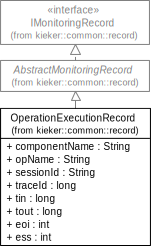
\includegraphics[scale=0.8]{images/kieker_OperationExecutionRecord-complete-modified}%
\caption{The class diagram of the operation execution record}
\label{fig:OperationExecutionRecordClassDiagramComplete}
\end{figure}

\enlargethispage{1cm}

\noindent Section~\ref{sec:traceMonitoring} describes how to instrument Java %
applications for monitoring trace information. %
It presents the technology-specific probes provided by \Kieker{} for this %
purpose---with a focus on AspectJ. %
Additional technology-specific probes can be implemented based on the existing %
probes. %
Section~\ref{sec:traceAnalysisTool} presents the %
tool which can be used to analyze and visualize the recorded trace %
data.  Examples for the available analysis and visualization outputs %
provided by \KiekerTraceAnalysis{} are presented in %
Section~\ref{sec:traceAnalysisExamples}.

\section{Monitoring Trace Information}\label{sec:traceMonitoring}

The following Sections describe how to use the monitoring probes based on %
AspectJ (Section~\ref{sec:traceAnalysis:instr:AspectJ}), %
the Java Servlet~API (Section~\ref{sec:traceAnalysis:instr:servlet}), %
the Spring Framework (Section~\ref{sec:traceAnalysis:instr:spring}), and %
Apache~CXF (Section~\ref{sec:traceAnalysis:instr:cxf}) provided %
by \Kieker{}. %

\subsection{AspectJ-Based Instrumentation}\label{sec:traceAnalysis:instr:AspectJ}

AspectJ~\cite{AspectJ-WebSite} allows to weave code into the byte code of %
Java applications and libraries without requiring manual modifications of the %
source code. %
\Kieker{} includes the AspectJ-based monitoring probes %
\class{OperationExecutionAspectAnnotation}, %
\class{OperationExecutionAspectAnnotationServlet}, %
\class{OperationExecutionAspectFull}, and %
\class{OperationExecutionAspectFullServlet} %
which can be woven into Java applications at compile time and load time. %
These probes monitor method executions and corresponding %
trace and timing information. The probes with the postfix \class{Servlet} %
additionally store a session identifier within the \class{OperationExecutionRecord}. %
When the probes with name element \class{Annotation} are used, %
methods to be monitored must be annotated by the \Kieker{} %
annotation \class{@OperationExecutionMonitoringProbe}. %
This section demonstrates how to use the AspectJ-based probes to monitor %
traces based on the Bookstore application from Chapter~\ref{chap:example}. %

\enlargethispage{1.0cm}

\NOTIFYBOX{The Java sources of the example presented in %
this section, as well as a pre-compiled binary, can be found in the %
\file{\aspectJBookstoreApplicationDirDistro{}/} directory of the %
binary release.}

% \

% This chapter will show in Section~\ref{sec:aspectJ:annotation} how
% to use AspectJ to mark methods to be monitored with a simple annotation
% in order to avoid the manual monitoring as seen in Chapter~\ref{chap:example}
% and \ref{chap:componentsMonitoring}. Once the methods are marked, the AspectJ-Weaver-Agent
% will surround the calls with the necessary code during runtime, similar
% to the manually inserted instrumentation code used in Section~\ref{sec:example:monitoring}.
% An alternative solution will be shown as well in Section~\ref{sec:aspectJ:fullweaving}, %
% where the methods to be instrumented are specified using an external configuration file %
% without requiring source code modifications. Both solutions
% can be used to reconstruct architectural views and to perform trace
% analyses. The result of both will be diagrams similar to sFigure~\ref{fig:bookstore:classAndSequenceDiagrams}.

% The idea of weaving the monitoring-code into the ``plain'' code
% during compile-time seems to suggest itself, but
% in this chapter it
% is only shown how to perform the so called load-time-weaving - the
% weaving during runtime.%, which is more flexible than the compile-time-weaving.

\begin{figure}[H]
\begin{graybox}
\dirtree{%
.1 \DirInDirTree{examples/}. %\DTcomment{The root directory of the project}.
.2 \DirInDirTree{userguide/}.
.3 \DirInDirTree{ch5--trace-monitoring-aspectj/}.
.4 \DirInDirTree{build/}\DTcomment{Directory for the Java class files}.
.5 \DirInDirTree{META-INF/}.
.4 \DirInDirTree{META-INF/} \DTcomment{Directory for the configuration files}.
.5 \newFileDirInDirTree{\aopConfigFile}.
.5 \kiekerMonitoringProperties{}.
.4 \DirInDirTree{lib/} \DTcomment{Directory for the needed libraries}.
.5 \newFileDirInDirTree{\mainJarWeaver}.
.4 \DirInDirTree{src/}\DTcomment{Directory for the source code files}.
.5 \DirInDirTree{bookstoreTracing/}.
.6 Bookstore.java.
.6 BookstoreStarter.java.
.6 Catalog.java.
.6 CRM.java.
}
\end{graybox}

\caption{The new directory structure of the Bookstore application}
\label{fig:bookstoreAOP:dirStructure}
\end{figure}

Figure~\ref{fig:bookstoreAOP:dirStructure} shows the directory used by the example of this section. %
The jar-file \file{\mainJarWeaver} already includes the \textit{AspectJ weaver}, %
which is registered with the JVM and weaves the monitoring instrumentation into %
the Java classes. It will be configured based on the configuration file %
\file{\file{\aopConfigFile}}, for which a working sample file is provided in the %
example's \dir{META-INF/} directory. Instead of registering the \file{\mainJarWeaver} %
as an agent to the JVM, the \file{\aspectJWeaverJar} can be used. In this case, %
the \file{\mainJar} needs to be added to the classpath.

Once the necessary files have been copied to the example directory, the source code can be instrumented with the annotation
\class{OperationExecutionMonitoringProbe}. Listing~\ref{lst:BookstoreAspectJ} shows how the annotation is used.

\setJavaCodeListing
\lstinputlisting[caption=Bookstore.java, label=lst:BookstoreAspectJ,firstline=21,firstnumber=21]{\aspectJBookstoreApplicationDir/src/kieker/examples/userguide/ch5bookstore/Bookstore.java}

\noindent As a first example, each method of the Bookstore application will be annotated. The annotation can be used to instrument all methods except for constructors.

The \file{\aopConfigFile} file has to be modified to specify the classes to be considered for instrumentation by the AspectJ weaver. Listing~\ref{lst:aopConfigFileAnnotations} shows the modified configuration file.

\enlargethispage{1cm}
\setXMLListing
\lstinputlisting[caption=aop.xml, label=lst:aopConfigFileAnnotations]{\aspectJBookstoreApplicationDir/META-INF/aop.xml}

\noindent Line~5 tells the AspectJ weaver to consider all classes inside the example package. %
AspectJ allows to use wild-cards for the definition of classes to %
include---e.g., \lstinline$<include within="bookstoreTracing.Bookstore*"/>$ to weave all %
classes with the prefix \class{Bookstore} located in a package \class{bookstoreTracing}.

Line~9 specifies the aspect to be woven into the classes. In this case, the \Kieker{} %
probe \class{OperationExecutionAspectAnnotation} is used. It requires that %
methods intended to be instrumented are annotated by %
\lstinline[language=Java]{@OperationExecutionMonitoringProbe}, as mentioned before.

Listings~\ref{lst:traceAnalysisCompileRunExample1} and %
\ref{lst:traceAnalysisCompileRunExample1Win} show how to compile and run the annotated %
Bookstore application. The \file{\aopConfigFile} must be located in a %
\dir{META-INF/} directory in the classpath---in this case the \dir{build/} directory. %
The AspectJ weaver has to be loaded as a so-called Java-agent. It weaves the %
monitoring aspect into the byte code of the Bookstore application. %
Additionally, a \file{\kiekerMonitoringProperties{}} is copied to the \dir{META-INF/} directory. %
This configuration file may be adjusted as desired (see Section~\ref{sec:monitoring:configuration}).

\


\setBashListing
\begin{lstlisting}[caption=Command to compile and run the instrumented Bookstore under Linux]
#\lstshellprompt{}# javac src/bookstoreTracing/Bookstore.java src/bookstoreTracing/CRM.java src/bookstoreTracing/Catalog.java src/bookstoreTracing/BookstoreStarter.java -d build/ -classpath lib/kieker-1.2-SNAPSHOT.jar:lib/commons-logging-1.1.1.jar

#\lstshellprompt{}# cp -r META-INF/aop.xml build/META-INF/aop.xml

#\lstshellprompt{}# java -javaagent:lib/aspectjweaver-1.6.9.jar -classpath build/:lib/kieker-1.2-SNAPSHOT.jar:lib/commons-logging-1.1.1.jar bookstoreTracing.BookstoreStarter
\end{lstlisting}

\begin{lstlisting}[caption=Commands to compile and run the annotated Bookstore under Windows, label=lst:traceAnalysisCompileRunExample1Win]
#\lstshellprompt{}# javac src/bookstoreTracing/Bookstore.java 
        src/bookstoreTracing/CRM.java 
        src/bookstoreTracing/Catalog.java 
        src/bookstoreTracing/BookstoreStarter.java 
        -d build/ 
        -classpath lib/#\mainJar{}#;lib/#\commonsLoggingJar{}#

#\lstshellprompt{}# copy META-INF\aop.xml build\META-INF\

#\lstshellprompt{}# java -#\textbf{javaagent:}#lib/#\aspectJWeaverJar{}# 
       -classpath build/;lib/#\mainJar{}#;lib/#\commonsLoggingJar{}# 
        bookstoreTracing.BookstoreStarter
\end{lstlisting}


\noindent After a complete run of the application, the monitoring files should appear in %
the same way as mentioned in Section~\ref{sec:example:monitoring} including the %
additional trace information. An example log of a complete run can be found in %
Appendix~\ref{sec:appendix:exampleConsoleOutputs:aspectJExample}.

\paragraph*{Instrumentation without annotations}%\label{sec:aspectJ:fullweaving}

AspectJ-based instrumentation without using annotations is quite simple. It is %
only necessary to modify the file \file{\aopConfigFile{}}, as shown %
in Listing~\ref{lst:aopConfigFileFull}.
\pagebreak
\setXMLListing
\lstinputlisting[caption=aop.xml, label=lst:aopConfigFileFull]{\aspectJBookstoreApplicationDir/META-INF/aop-full.xml}

\noindent The alternative aspect \class{OperationExecutionAspectFull} is being %
activated in line~9. As indicated by its name, this aspect makes sure that every %
method within the included classes/packages will be instrumented and monitored. %
% The exact behavior can be controlled very exactly by using appropriate includes and excludes within the weaver-part of the configuration file. %
% For example,
Listing \ref{lst:aopConfigFileFull} demonstrates how to limit the %
instrumented methods to those of the class \class{BookstoreStarter}.

The commands shown in the Listings~\ref{lst:traceAnalysisCompileRunExample1} and %
\ref{lst:traceAnalysisCompileRunExample1Win} can again be used to compile and execute %
the example. Note that the annotations within the source code have no effect %
when using this aspect.

\

\WARNBOX{When using a custom aspect, it can be necessary to specify its %
classname in the \lstinline{include} directives of the \aopConfigFile{}.}

\subsection{Servlet Filters}\label{sec:traceAnalysis:instr:servlet}

The Java Servlet API~\cite{JavaServletTechnology-WebSite} includes the %
\class{javax.servlet.Filter} interface. It can be used to implement %
interceptors for incoming HTTP requests. %
\Kieker{} includes the probe %
\class{SessionAndTraceRegistrationFilter} which implements the %
\class{javax.servlet.Filter} interface. %
It initializes the session and trace information for incoming requests. %
If desired, it additionally creates an \class{OperationExecutionRecord} for each %
invocation of the filter and passes it to the \class{MonitoringController}.

% \enlargethispage{1.5cm}

Listing~\ref{lst:OperationExecutionRegistrationAndLoggingFilterInWebXML} %
demonstrates how to integrate the \class{SessionAndTraceRegistrationFilter} %
in the \file{web.xml} file of a web application.

The Java~EE Servlet container example described in Appendix~\ref{appendix:JavaEEServletExample} employs the %
\class{SessionAndTraceRegistrationFilter}.

\pagebreak

\setXMLListing
\lstinputlisting[firstline=50,lastline=61,firstnumber=50,%
caption=\class{SessionAndTraceRegistrationFilter} in a \file{web.xml} file,%
label=lst:OperationExecutionRegistrationAndLoggingFilterInWebXML]%
{\JavaEEServletExampleDir/jetty/webapps/jpetstore/WEB-INF/web.xml}


\subsection{Spring}\label{sec:traceAnalysis:instr:spring}

The Spring framework~\cite{Spring-WebSite} provides interfaces for intercepting %
Spring services and web requests. %
\Kieker{} includes the probes %
\class{OperationExecutionMethodInvocationInterceptor} and
\class{OperationExecutionWebRequestRegistrationInterceptor}. %
The \class{OperationExecutionMethodInvocationInterceptor} is similar to the %
AspectJ-based probes described in the previous section and monitors method %
executions as well as corresponding trace and session information. %
The \class{OperationExecutionWebRequestRegistrationInterceptor} intercepts %
incoming Web requests and initializes the trace and session data for this %
trace. If you are not using the \class{OperationExecutionWebRequestRegistrationInterceptor}, %
you should use one of the previously described Servlet filters to register %
session information for incoming requests %
(Section~\ref{sec:traceAnalysis:instr:servlet}).

See the Spring documentation for instructions how to add the interceptors %
to the server configuration.

\subsection{CXF SOAP Interceptors}\label{sec:traceAnalysis:instr:cxf}

The Apache~CXF framework~\cite{CXF-WebSite} allows to implement interceptors for web service calls, %
for example, based on the SOAP web service protocol. %
\Kieker{} includes the probes %
\class{OperationExecutionSOAPRequestOutInterceptor}, %
\class{OperationExecutionSOAPRequestInInterceptor}, %
\class{OperationExecutionSOAPResponseOutInterceptor}, and %
\class{OperationExecutionSOAPResponseInInterceptor} which can be used to %
monitor SOAP-based web service calls. %
Session and trace information is written to and read from the SOAP header of %
service requests and responses allowing to monitor distributed traces. %
See the CXF documentation for instructions how to add the interceptors %
to the server configuration.

\pagebreak

\section{Trace Analysis and Visualization}\label{sec:traceAnalysisTool}

\enlargethispage{0.5cm}

Monitoring data including trace information can be analyzed and visualized with the \KiekerTraceAnalysis{} tool which is included in the \Kieker{} binary as well.\\

\WARNBOX{
In order to use this tool, it is necessary to install two third-party programs:
\begin{enumerate}
\item \textbf{Graphviz} A graph visualization software which can be downloaded from \url{http://www.graphviz.org/}.
\item \textbf{GNU PlotUtils} A set of tools for generating 2D plot graphics which can be downloaded from \url{http://www.gnu.org/software/plotutils/} (for Linux) and from \url{http://gnuwin32.sourceforge.net/packages/plotutils.htm} (for Windows).
\item \textbf{ps2pdf} The \file{ps2pdf} tool is used to convert ps files to pdf files.
\end{enumerate}
Under Windows it is recommended to add the \dir{bin/} directories of both tools to the ``path'' environment variable. It is also possible that the GNU PlotUtils are unable to process sequence diagrams. In this case it is recommended to use the Cygwin port of PlotUtils.
}

\vspace{1mm}

\noindent Once both programs have been installed, the \KiekerTraceAnalysis{} tool can be used. It can be accessed via the wrapper-script \file{trace-analysis.sh} or \file{trace-analysis.bat} (Windows) in the \dir{bin/} directory. Non-parameterized calls of the scripts print all possible options on the screen, as listed in Appendix~\ref{appendix:wrapperScripts:traceAnalysis}.

The commands shown in Listings~\ref{lst:traceAnalysis:sequenceDiagram} and \ref{lst:traceAnalysis:sequenceDiagramWin} generate a sequence diagram as well as a call tree to an existing directory named \dir{out/}. The monitoring data is assumed to be located in the directory \dir{/tmp/kieker-20110428-142829399-UTC-Kaapstad-KIEKER/} or \dir{\%temp\%$\backslash{}$kieker-20100813-121041532-UTC-virus-KIEKER} under Windows. %

\setBashListing
\begin{lstlisting}[caption=Commands to produce the diagrams under \UnixLikeSystems,label=lst:traceAnalysis:sequenceDiagram]
#\lstshellprompt{}# #\textbf{./trace-analysis.sh}# #\textbf{--inputdirs}# /tmp/kicker-20110428-142829399-UTC-Kaapstad-KIEKER
                     #\textbf{--outputdir}# out/
                     #\textbf{--plot-Deployment-Sequence-Diagrams}#
                     #\textbf{--plot-Call-Trees}#							 
\end{lstlisting}

\begin{lstlisting}[caption=Commands to produce the diagrams under Windows,label=lst:traceAnalysis:sequenceDiagramWin]
#\lstshellprompt{}# #\textbf{trace-analysis.bat}# #\textbf{--inputdirs}# %temp%\kieker-20100813-121041532-UTC-virus-KIEKER
                    #\textbf{--outputdir}# out\
                    #\textbf{--plot-Deployment-Sequence-Diagrams}#
                    #\textbf{--plot-Call-Trees}#		
\end{lstlisting}


\enlargethispage{1cm}

\WARNBOX{%
The Windows \file{.bat} wrapper scripts (including \file{trace-analysis.bat}) must be executed from within %
the \dir{bin/} directory.
}

\pagebreak

The resulting contents of the \dir{out/} directory should be similar to %
the following tree:

\begin{figure}[H]
\begin{graybox}
\dirtree{%
.1 \DirInDirTree{out/}.
.2 deploymentSequenceDiagram-6120391893596504065.pic.
.2 callTree-6120391893596504065.dot.
.2 system-entities.html.
}
\end{graybox}
\end{figure}

\noindent The \file{.pic} and \file{.dot} files can be converted into other formats, %
such as \file{.pdf}, by using the \textit{Graphviz} and \textit{PlotUtils} tools %
\file{dot} and \file{pic2plot}. %
The following Listing~\ref{lst:traceAnalysis:convertDiagrams} demonstrates this. %

% The generated diagrams are shown in the following %
% Figures~\ref{fig:traceAnalysis:callTree} and~\ref{fig:traceAnalysis:allocSeqDiagr}.

\begin{lstlisting}[caption=Commands to convert the diagrams,label=lst:traceAnalysis:convertDiagrams]
#\lstshellprompt{}# dot callTree-6120391893596504065.dot #\textbf{-T}png# #\textbf{-o}# callTree.png
#\lstshellprompt{}# pic2plot deploymentSequenceDiagram-6120391893596504065.pic #\textbf{-T}png# > sequenceDiagram.png			 
\end{lstlisting}

% \begin{figure}[H]\centering
%   \subfigure[]{\label{fig:traceAnalysis:callTree}%
%   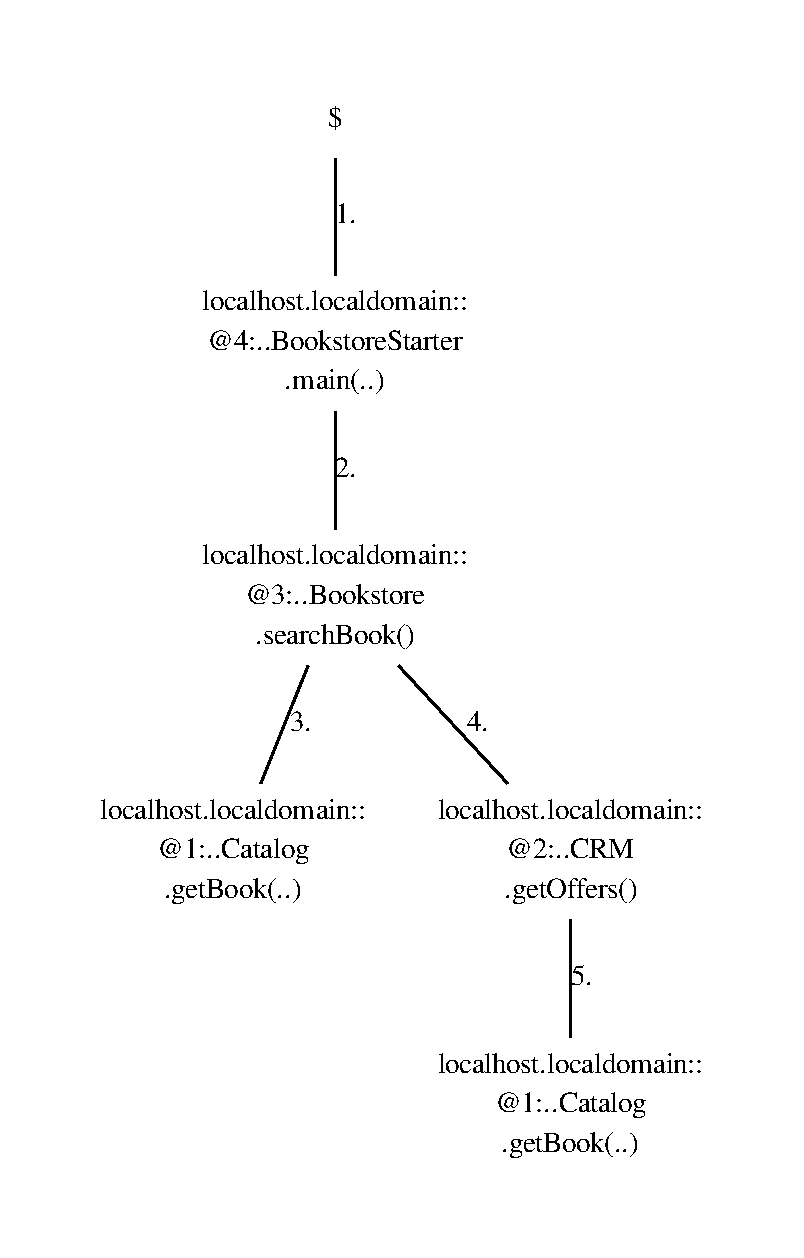
\includegraphics[height=0.4\textheight]{images/callTree}
%   }%
%   \subfigure[]{\label{fig:traceAnalysis:allocSeqDiagr}%
%   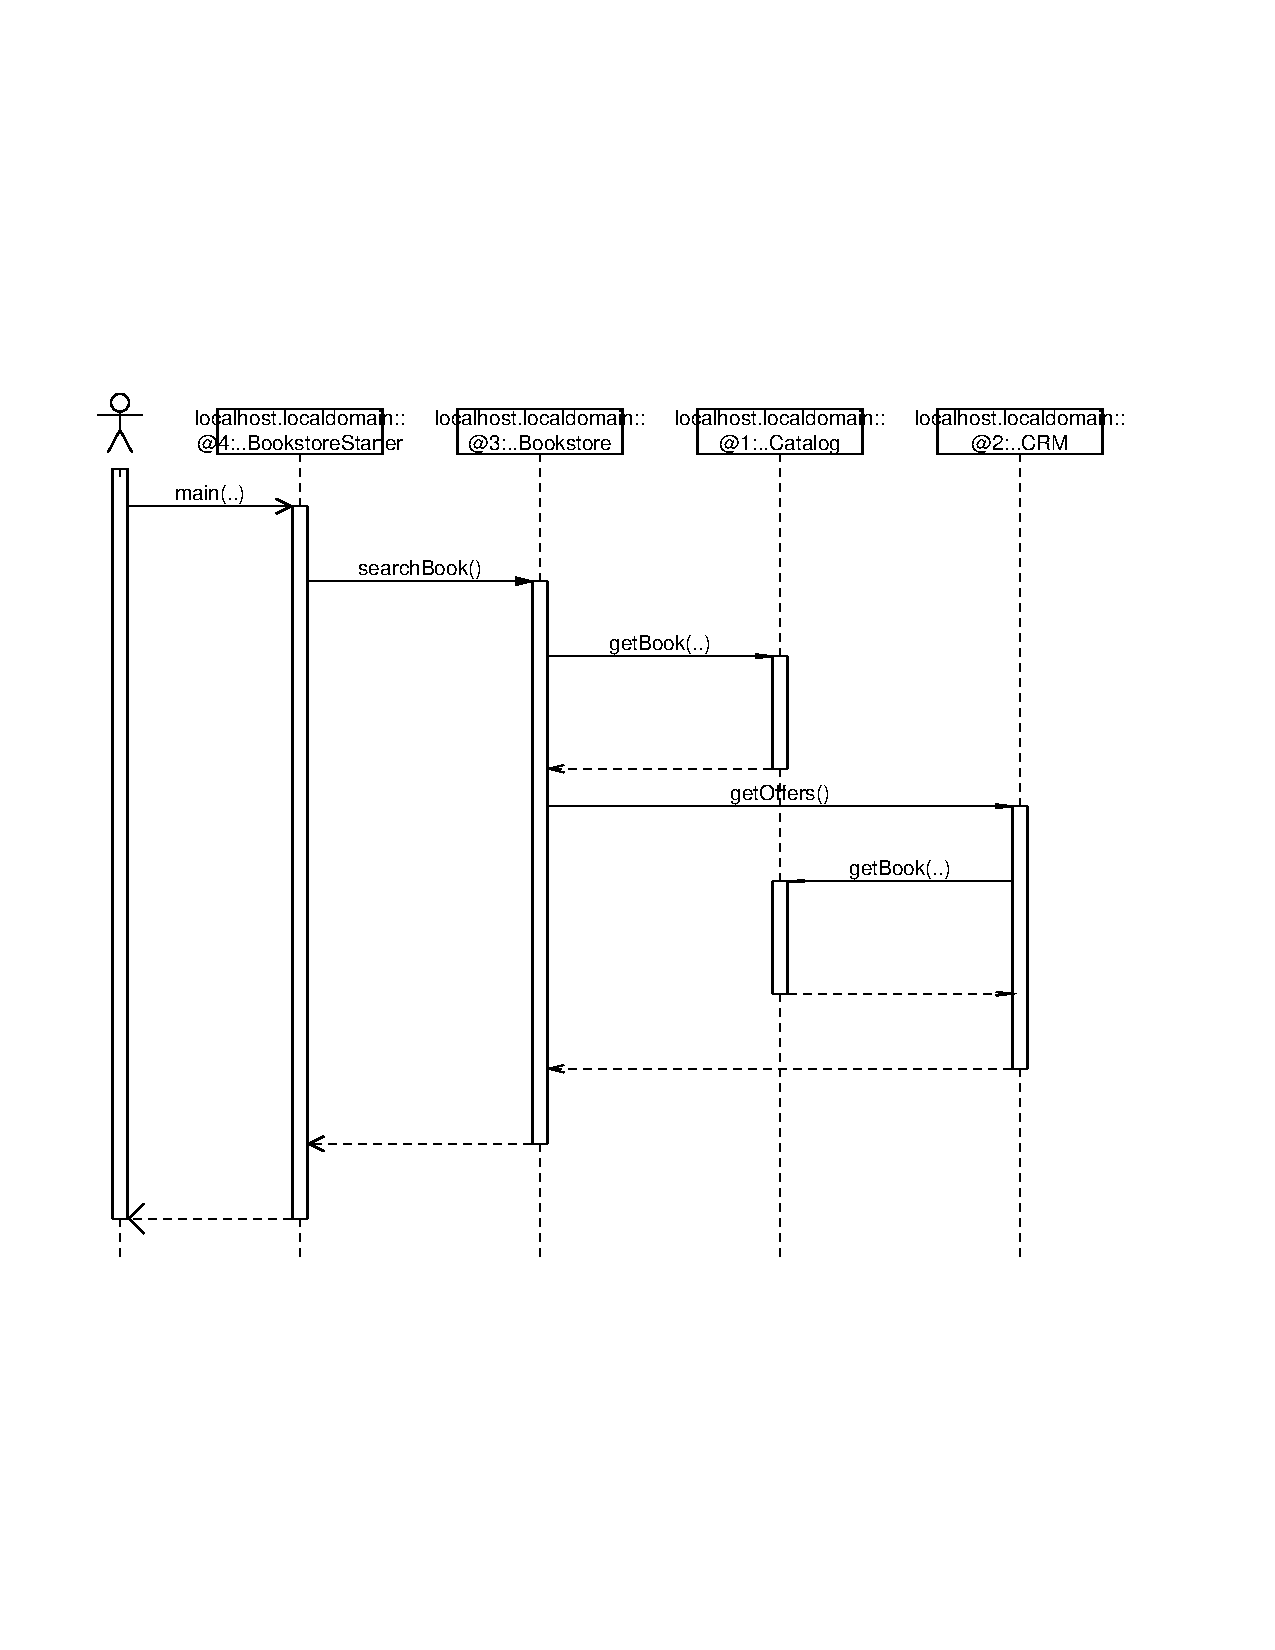
\includegraphics[height=0.4\textheight]{images/allocationSequenceDiagram}
%   }%
%
%   \caption{Call Tree~\subref{fig:traceAnalysis:callTree} and Allocation Sequence Diagram~\subref{fig:traceAnalysis:allocSeqDiagr}}
% \end{figure}

\NOTIFYBOX{The scripts \file{dotPic-fileConverter.sh} and \file{dotPic-fileConverter.bat} %
convert all \file{.pic} and \file{.dot} in a specified directory. %
See Appendix~\ref{appendix:wrapperScripts:dotPicFileConverter} for details.}

\vspace{5mm}

Examples of all available visualization are presented in the following %
Section~\ref{sec:traceAnalysisExamples}.

\pagebreak

\section{Example \KiekerTraceAnalysis{} Outputs}\label{sec:traceAnalysisExamples}
\newcommand{\OPT}[1]{\texttt{#1}}
\newcommand{\OPTprintValidExecutionTraces}{-\,-print-Execution-Traces}
\newcommand{\OPTprintInvalidExecutionTraces}{-\,-print-invalid-Execution-Traces}
\newcommand{\OPTprintMessageTraces}{-\,-print-Message-Traces}
\newcommand{\OPTprintDeploymentEquivalenceClasses}{-\,-print-Deployment-Equivalence-Classes}
\newcommand{\OPTprintAssemblyEquivalenceClasses}{-\,-print-Assembly-Equivalence-Classes}
\newcommand{\OPTplotDeploymentSequenceDiagrams}{-\,-plot-Deployment-Sequence-Diagrams}
\newcommand{\OPTplotAssemblySequenceDiagrams}{-\,-plot-Assembly-Sequence-Diagrams}
\newcommand{\OPTplotCallTrees}{-\,-plot-Call-Trees}
\newcommand{\OPTplotAggregatedDeploymentCallTree}{-\,-plot-Aggregated-Deployment-Call-Tree}
\newcommand{\OPTplotAggregatedAssemblyCallTree}{-\,-plot-Aggregated-Assembly-Call-Tree}

\newcommand{\OPTplotContainerDependencyGraph}{-\,-plot-Container-Dependency-Graph}
\newcommand{\OPTplotDeploymentComponentDependencyGraph}{-\,-plot-Deployment-Component-Dependency-Graph}
\newcommand{\OPTplotAssemblyComponentDependencyGraph}{-\,-plot-Assembly-Component-Dependency-Graph}
\newcommand{\OPTplotDeploymentOperationDependencyGraph}{-\,-plot-Deployment-Operation-Dependency-Graph}
\newcommand{\OPTplotAssemblyOperationDependencyGraph}{-\,-plot-Assembly-Operation-Dependency-Graph}

The examples presented in this section were generated based on the %
monitoring data which can be found in the directory %
\dir{\distributedTestdataDirDistro/}. It consists of 1635 traces %
of the Bookstore application with AspectJ-based instrumentation, %
as described in Section~\ref{sec:traceAnalysis:instr:AspectJ}. %
In order to illustrate the visualization of distributed traces, %
the hostname of the \class{Catalog}'s method \method{getBook} was %
probabilistically changed to a second hostname. %
For a more detailed description of the underlying formalisms, %
we refer to our technical report~\cite{vanHoornRohrHasselbringWallerEhlersFreyKieselhorst2009TRContinuousMonitoringOfSoftwareServicesDesignAndApplicationOfTheKiekerFramework}. %
The output can be found in the directory %
\dir{\distributedTestdataDirDistro-example-plots/}.

\subsection{Textual Trace and Equivalence Class Representations}

\subsubsection{Execution Traces}\label{sec:example:executionTraces}%

Textual execution trace representations of valid/invalid traces are written to %
an output file using the command-line options \OPT{\OPTprintValidExecutionTraces} and %
\OPT{\OPTprintInvalidExecutionTraces}. %
Listing~\ref{lst:appendix:traceAnalysisExample:executionTraces} %
shows the execution trace representation for the valid trace \ldots6129.

\setTextListing
\lstinputlisting[firstline=1,lastline=5,escapechar={},%
caption=Textual output of trace 6488138950668976129's execution trace representation,%
label=lst:appendix:traceAnalysisExample:executionTraces]%
{../../examples/userguide/ch5--trace-monitoring-aspectj/testdata/kieker-20100830-082225522-UTC-example-plots/executionTraces.txt} % macros don't work here ...

\subsubsection{Message Traces}\label{sec:example:messageTraces}%

Textual message trace representations of valid traces are written to an output %
file using the command-line option \OPT{\OPTprintMessageTraces}. %
Listing~\ref{lst:appendix:traceAnalysisExample:messageTraces} %
shows the message trace representation for the valid trace \ldots6129.

\setTextListing
\lstinputlisting[firstline=1,lastline=9,escapechar={},%
caption=Textual output of trace 6488138950668976129's message trace representation,%
label=lst:appendix:traceAnalysisExample:messageTraces]%
{../../examples/userguide/ch5--trace-monitoring-aspectj/testdata/kieker-20100830-082225522-UTC-example-plots/messageTraces.txt}

\subsubsection{Trace Equivalence Classes}\label{sec:example:traceEquivClasses}%

Deployment/assembly-level trace equivalence classes are computed and written %
to output files using the command-line options \OPT{\OPTprintDeploymentEquivalenceClasses} %
and \OPT{\OPTprintAssemblyEquivalenceClasses}. %
Listings~\ref{lst:appendix:traceAnalysisExample:traceDeploymentEquivClasses} and %
\ref{lst:appendix:traceAnalysisExample:traceAssemblyEquivClasses} show the %
output generated for the monitoring data used in this section. %

\setTextListing
\lstinputlisting[caption=Textual output of information on the \textit{deployment-level} trace equivalence classes,%
label=lst:appendix:traceAnalysisExample:traceDeploymentEquivClasses]
{../../examples/userguide/ch5--trace-monitoring-aspectj/testdata/kieker-20100830-082225522-UTC-example-plots/traceDeploymentEquivClasses.txt}

\setTextListing
\lstinputlisting[caption=Textual output of information on the \textit{assembly-level} trace equivalence class,%
label=lst:appendix:traceAnalysisExample:traceAssemblyEquivClasses]%
{../../examples/userguide/ch5--trace-monitoring-aspectj/testdata/kieker-20100830-082225522-UTC-example-plots/traceAssemblyEquivClasses.txt}

\pagebreak

\subsection{Sequence Diagrams}\label{sec:example:seqDiagrams}%

\subsubsection{Deployment-Level Sequence Diagrams}\label{sec:example:deploymentSeqDiagrams}%

Deployment-level sequence diagrams are generated using the command-line option \OPT{\OPTplotDeploymentSequenceDiagrams}. %
Figures~\ref{fig:appendix:traceAnalysisExample:SeqDiagrsDepl6129}--\ref{fig:appendix:traceAnalysisExample:SeqDiagrsDepl6141} %
show these sequence diagrams for each deployment-level %
trace equivalence representative (Section~\ref{sec:example:traceEquivClasses}).

\begin{figure}[h]\centering
\subfigure[Trace \ldots{}6129]{\label{fig:appendix:traceAnalysisExample:SeqDiagrsDepl6129}%
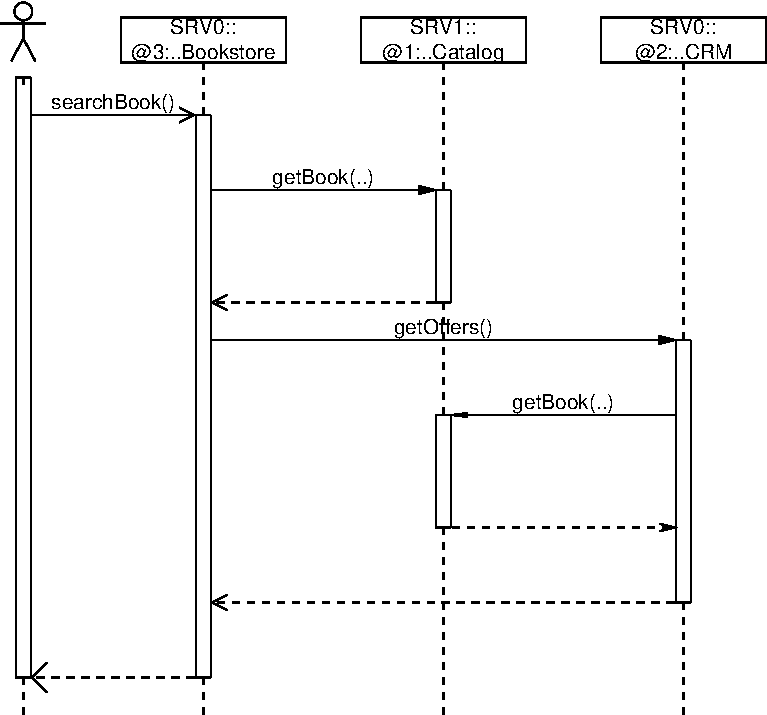
\includegraphics[scale=0.39]{../../examples/userguide/ch5--trace-monitoring-aspectj/testdata/kieker-20100830-082225522-UTC-example-plots/deploymentSequenceDiagram-6488138950668976129-crop}
}
\subfigure[Trace \ldots{}6130]{\label{fig:appendix:traceAnalysisExample:SeqDiagrsDepl6130}%
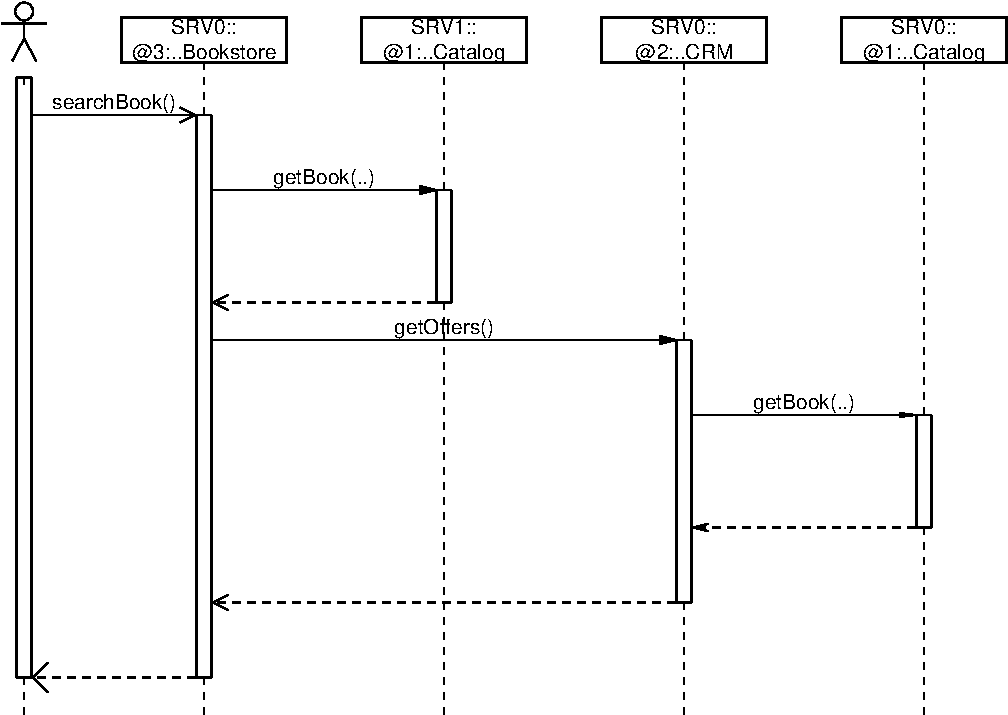
\includegraphics[scale=0.39]{../../examples/userguide/ch5--trace-monitoring-aspectj/testdata/kieker-20100830-082225522-UTC-example-plots/deploymentSequenceDiagram-6488138950668976130-crop}
}
\subfigure[Trace \ldots{}6131]{\label{fig:appendix:traceAnalysisExample:SeqDiagrsDepl6131}%
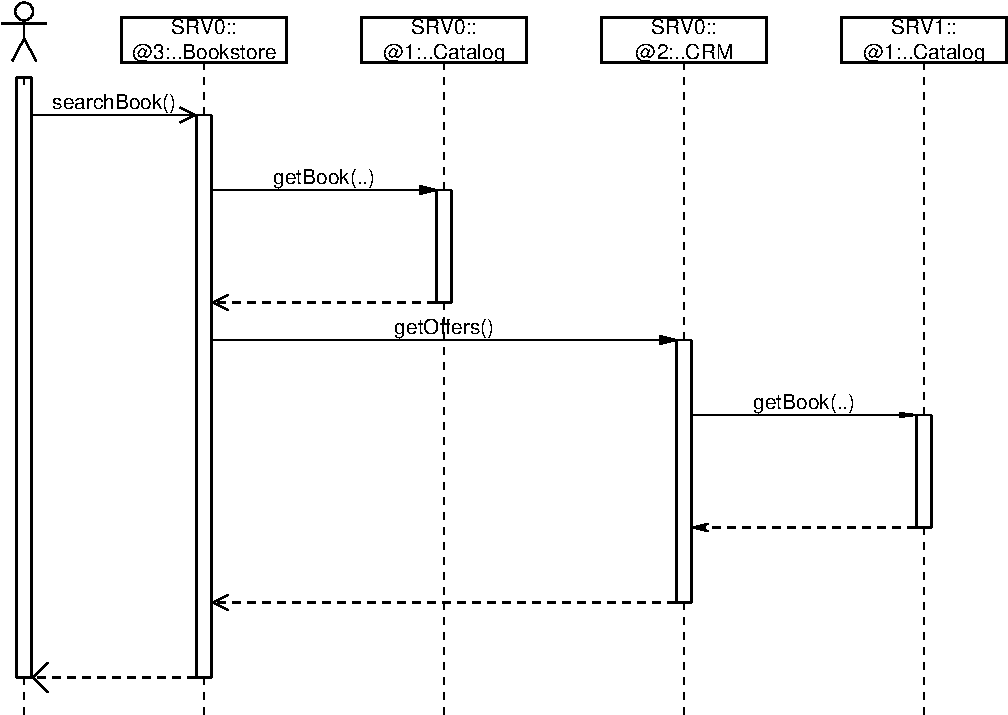
\includegraphics[scale=0.39]{../../examples/userguide/ch5--trace-monitoring-aspectj/testdata/kieker-20100830-082225522-UTC-example-plots/deploymentSequenceDiagram-6488138950668976131-crop}
}
\subfigure[Trace \ldots{}6141]{\label{fig:appendix:traceAnalysisExample:SeqDiagrsDepl6141}%
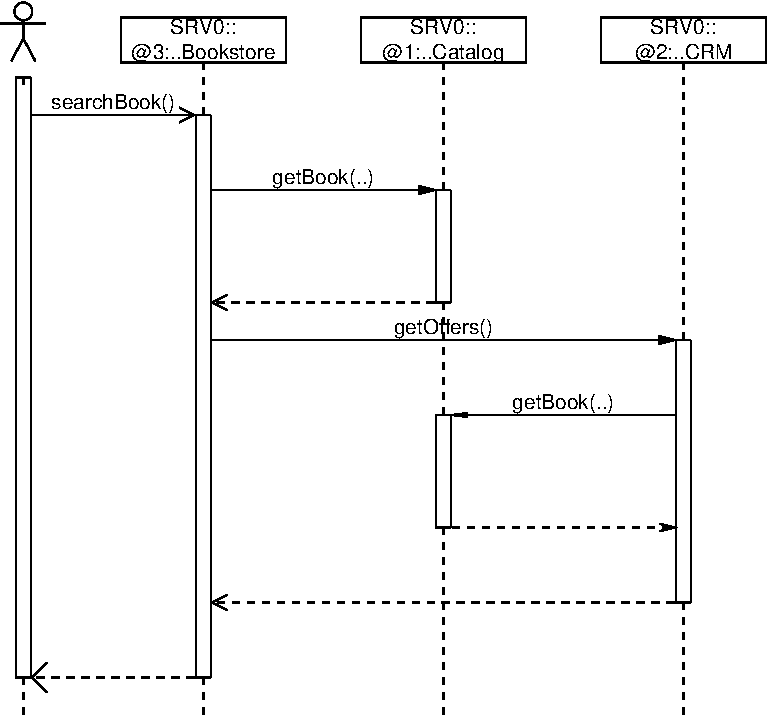
\includegraphics[scale=0.39]{../../examples/userguide/ch5--trace-monitoring-aspectj/testdata/kieker-20100830-082225522-UTC-example-plots/deploymentSequenceDiagram-6488138950668976141-crop}
}
\caption{\textit{Deployment-level} sequence diagrams of the trace %
equivalence class representatives (Listing~\ref{lst:appendix:traceAnalysisExample:traceAssemblyEquivClasses})}
\label{fig:appendix:traceAnalysisExample:SeqDiagrsDepl}
\end{figure}

% \enlargethispage{2cm}
\pagebreak

\subsubsection{Assembly-Level Sequence Diagrams}\label{sec:example:assemblySeqDiagrams}%

Assembly-level sequence diagrams are generated using the command-line option \OPT{\OPTplotAssemblySequenceDiagrams}. %
Figure~\ref{fig:appendix:traceAnalysisExample:SeqDiagrDepl6129} %
shows the sequence diagram for the assembly-level trace equivalence representative %
(Section~\ref{sec:example:traceEquivClasses}).

\begin{figure}[h]\centering
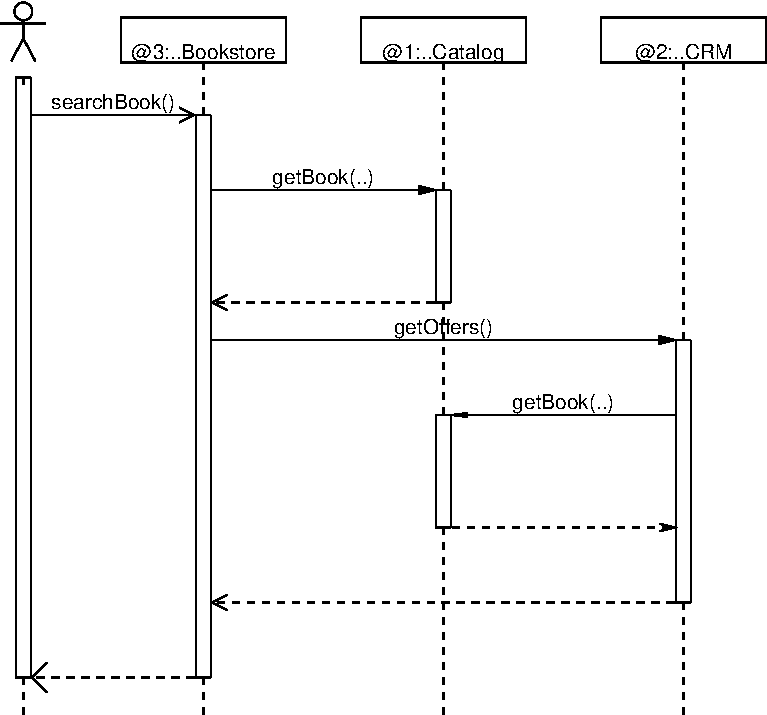
\includegraphics[scale=0.39]{../../examples/userguide/ch5--trace-monitoring-aspectj/testdata/kieker-20100830-082225522-UTC-example-plots/assemblySequenceDiagram-6488138950668976129-crop}
\caption{\textit{Assembly-level} sequence diagram of trace \ldots{}6129}
\label{fig:appendix:traceAnalysisExample:SeqDiagrDepl6129}
\end{figure}

% \pagebreak

\subsection{Call Trees}\label{sec:example:callTrees}%

\subsubsection{Trace Call Trees}\label{sec:example:traceCallTrees}%

\enlargethispage{1.2cm}

Trace call trees are generated using the command-line option \OPT{\OPTplotCallTrees}. %
Figures~\ref{fig:appendix:traceAnalysisExample:TraceCallTrees6129}--\ref{fig:appendix:traceAnalysisExample:TraceCallTrees6141} %
show these call trees for each deployment-level %
trace equivalence representative (Section~\ref{sec:example:traceEquivClasses}).

\begin{figure}[h]\centering
\subfigure[Trace \ldots{}6129]{\label{fig:appendix:traceAnalysisExample:TraceCallTrees6129}%
\ \ 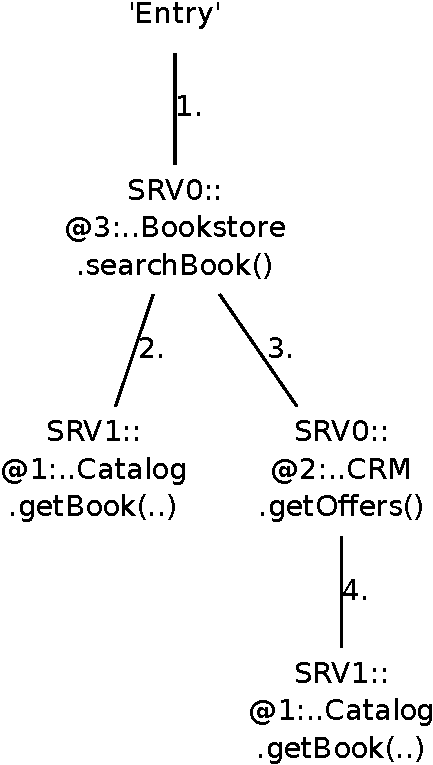
\includegraphics[scale=0.4]{../../examples/userguide/ch5--trace-monitoring-aspectj/testdata/kieker-20100830-082225522-UTC-example-plots/callTree-6488138950668976129-crop}\ \ 
}
\subfigure[Trace \ldots{}6130]{\label{fig:appendix:traceAnalysisExample:TraceCallTrees6130}%
\ \ 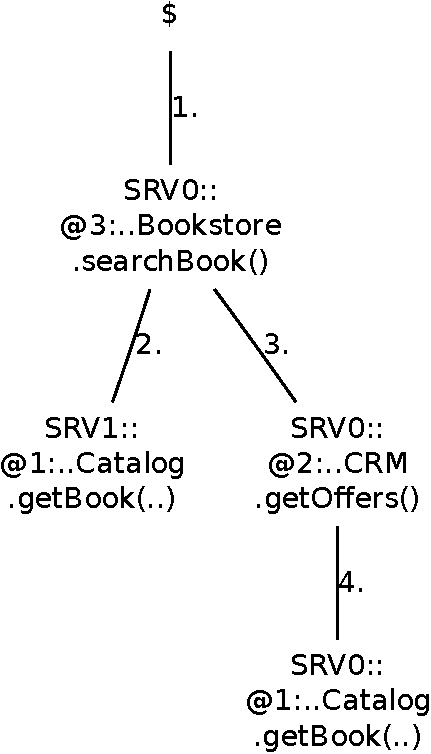
\includegraphics[scale=0.4]{../../examples/userguide/ch5--trace-monitoring-aspectj/testdata/kieker-20100830-082225522-UTC-example-plots/callTree-6488138950668976130-crop}\ \ 
}
\subfigure[Trace \ldots{}6131]{\label{fig:appendix:traceAnalysisExample:TraceCallTrees6131}%
\ \ 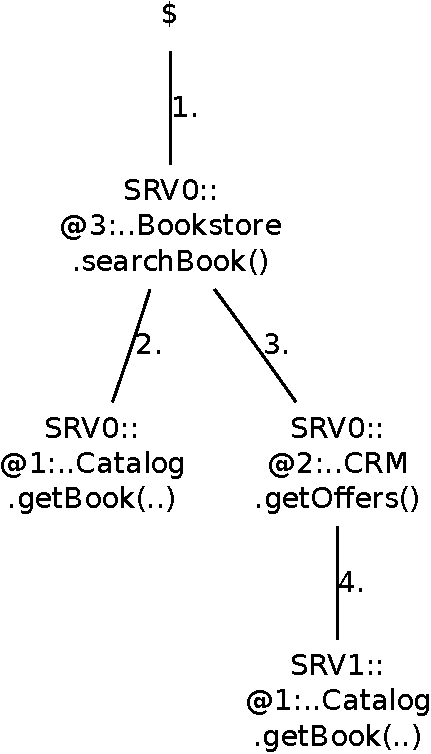
\includegraphics[scale=0.4]{../../examples/userguide/ch5--trace-monitoring-aspectj/testdata/kieker-20100830-082225522-UTC-example-plots/callTree-6488138950668976131-crop}\ \ 
}
\subfigure[Trace \ldots{}6141]{\label{fig:appendix:traceAnalysisExample:TraceCallTrees6141}%
\ \ 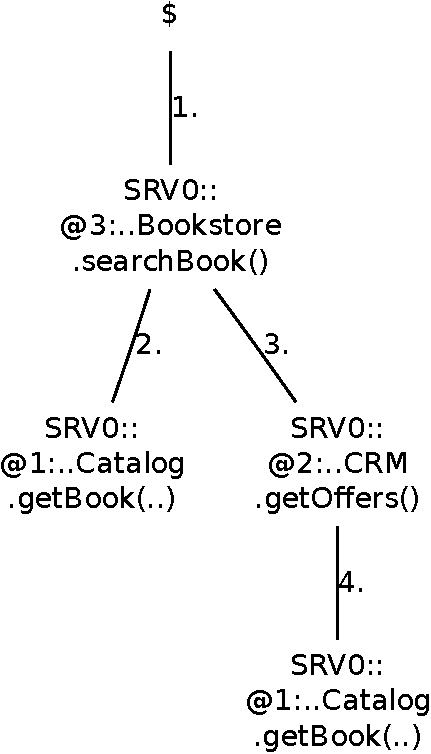
\includegraphics[scale=0.4]{../../examples/userguide/ch5--trace-monitoring-aspectj/testdata/kieker-20100830-082225522-UTC-example-plots/callTree-6488138950668976141-crop}\ \ 
}
\caption{Calls trees of the trace %
equivalence class representatives (Listing~\ref{lst:appendix:traceAnalysisExample:traceAssemblyEquivClasses})}
\label{fig:appendix:traceAnalysisExample:TraceCallTrees}
\end{figure}

% \newpage

\subsubsection{Aggregated Call Trees}\label{sec:example:aggregatedCallTrees}%

Aggregated deployment/assembly-level call trees are generated using the command-line options %
\OPT{\OPTplotAggregatedDeploymentCallTree} and \OPT{\OPTplotAggregatedAssemblyCallTree}. %
Figures~\ref{fig:appendix:traceAnalysisExample:AggregatedCallTreesDeployment} and \ref{fig:appendix:traceAnalysisExample:AggregatedCallTreesAssembly} %
show these aggregated call trees for the traces contained in the monitoring data %
used in this section. %

\begin{figure}[h]\centering
\subfigure[deployment-level]{\label{fig:appendix:traceAnalysisExample:AggregatedCallTreesDeployment}%
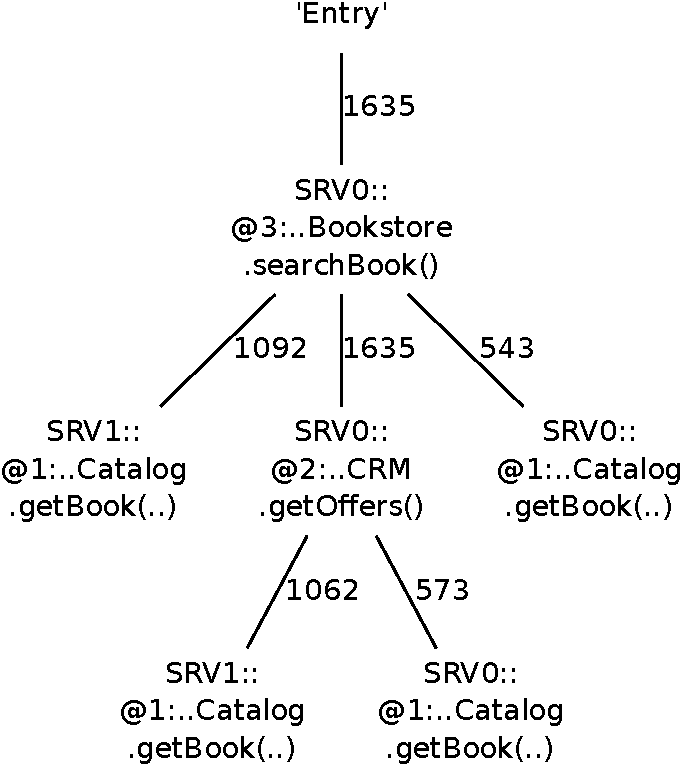
\includegraphics[scale=0.4]{../../examples/userguide/ch5--trace-monitoring-aspectj/testdata/kieker-20100830-082225522-UTC-example-plots/aggregatedDeploymentCallTree-crop}%
}
\subfigure[assembly-level]{\label{fig:appendix:traceAnalysisExample:AggregatedCallTreesAssembly}%
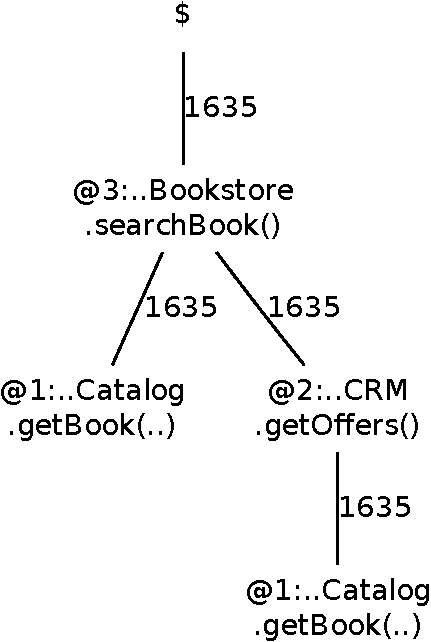
\includegraphics[scale=0.4]{../../examples/userguide/ch5--trace-monitoring-aspectj/testdata/kieker-20100830-082225522-UTC-example-plots/aggregatedAssemblyCallTree-crop}%
}
\caption{Aggregated call trees generated from the 1635~traces}
\label{fig:appendix:traceAnalysisExample:AggregatedCallTrees}
\end{figure}

\pagebreak

\subsection{Dependency Graphs}

\subsubsection{Container Dependency Graphs}

A container dependency graph is generated using the command-line option %
\OPT{\OPTplotContainerDependencyGraph}. %
Figure~\ref{fig:appendix:traceAnalysisExample:ContainerDepGraph} shows the %
container dependency graph for the monitoring data used in this section. 

\begin{figure}[h]\centering
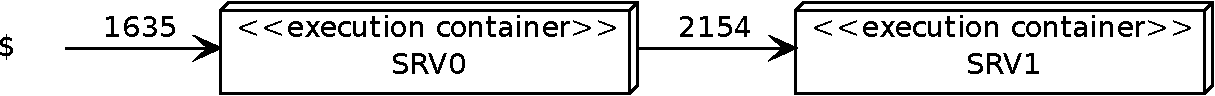
\includegraphics[scale=0.45]{../../examples/userguide/ch5--trace-monitoring-aspectj/testdata/kieker-20100830-082225522-UTC-example-plots/containerDependencyGraph-crop}
\caption{Container dependency graph}
\label{fig:appendix:traceAnalysisExample:ContainerDepGraph}
\end{figure}

\subsubsection{Component Dependency Graphs}

Deployment/assembly-level component dependency graphs are generated using the %
command-line options \OPT{\OPTplotDeploymentComponentDependencyGraph} and %
\OPT{\OPTplotAssemblyComponentDependencyGraph}. %
Figures~\ref{fig:appendix:traceAnalysisExample:ComponentDepGraphsDeployment} and %
\ref{fig:appendix:traceAnalysisExample:ComponentDepGraphsAssembly} show the %
component dependency graphs for the monitoring data used in this section. 

\begin{figure}[h]\centering
\subfigure[deployment-level]{\label{fig:appendix:traceAnalysisExample:ComponentDepGraphsDeployment}%
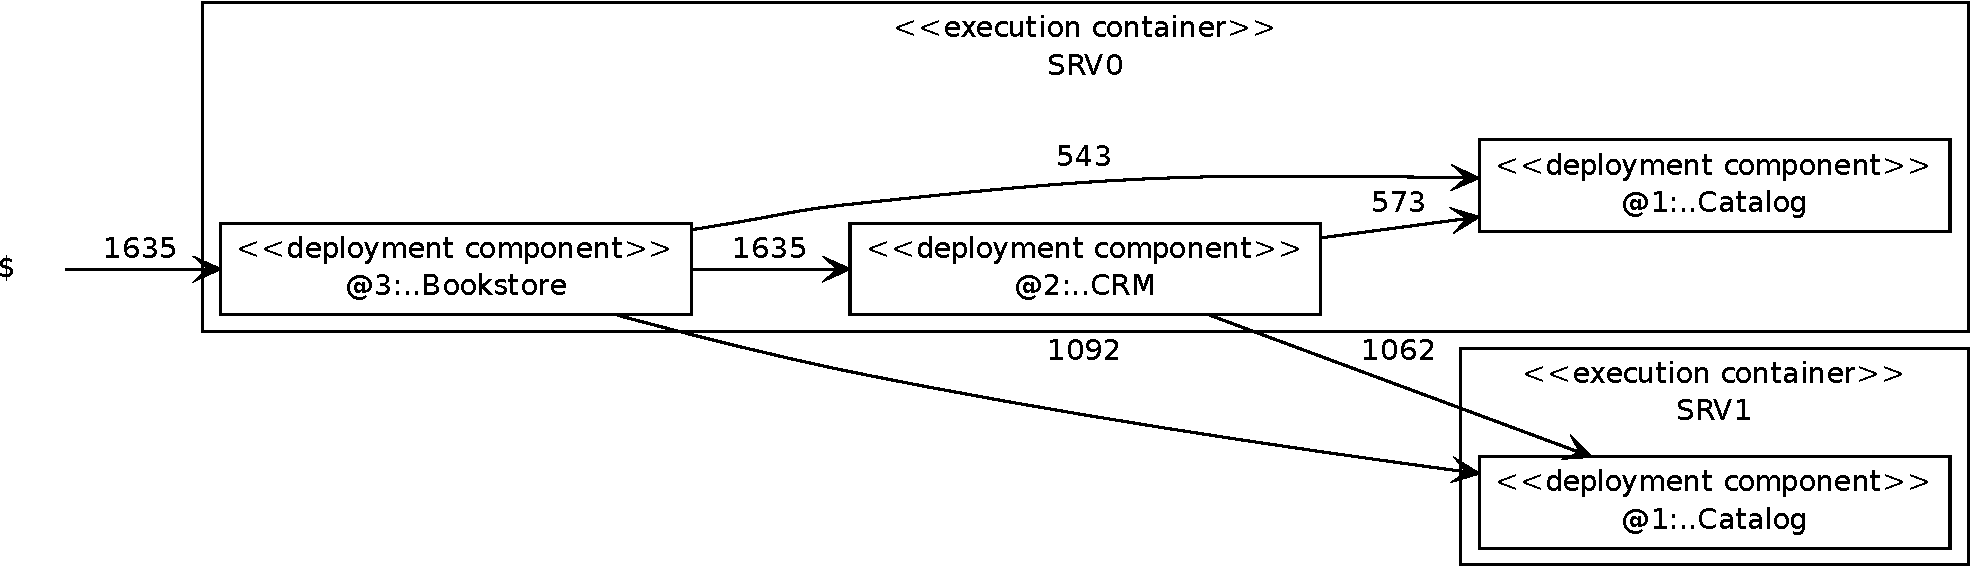
\includegraphics[scale=0.45]{../../examples/userguide/ch5--trace-monitoring-aspectj/testdata/kieker-20100830-082225522-UTC-example-plots/deploymentComponentDependencyGraph-crop}
}
\subfigure[assembly-level]{\label{fig:appendix:traceAnalysisExample:ComponentDepGraphsAssembly}%
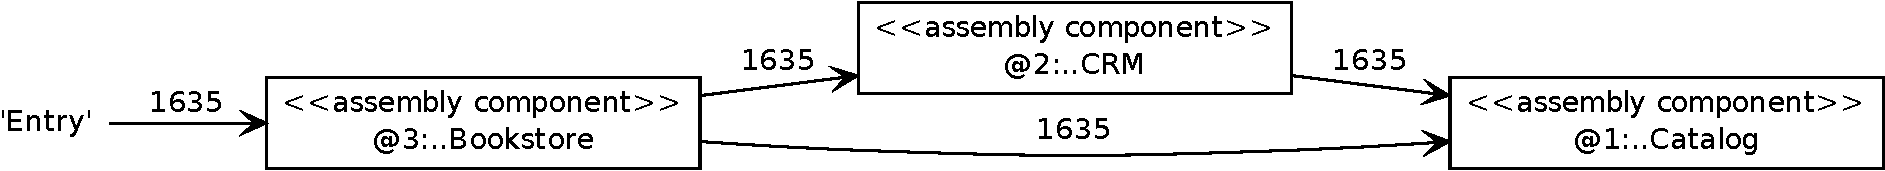
\includegraphics[scale=0.45]{../../examples/userguide/ch5--trace-monitoring-aspectj/testdata/kieker-20100830-082225522-UTC-example-plots/assemblyComponentDependencyGraph-crop}
}
\caption{Component dependency graphs}
\label{fig:appendix:traceAnalysisExample:ComponentDepGraphs}
\end{figure}

\pagebreak

\subsubsection{Operation Dependency Graphs}

Deployment/assembly-level operation dependency graphs are generated using the %
command-line options \OPT{\OPTplotDeploymentOperationDependencyGraph} and %
\OPT{\OPTplotAssemblyOperationDependencyGraph}. %
Figures~\ref{fig:appendix:traceAnalysisExample:OperationDepGraphsDeployment} and %
\ref{fig:appendix:traceAnalysisExample:OperationDepGraphsAssembly} show the %
operation dependency graphs for the monitoring data used in this section. 

\begin{figure}[ht]\centering
\subfigure[deployment-level]{\label{fig:appendix:traceAnalysisExample:OperationDepGraphsDeployment}%
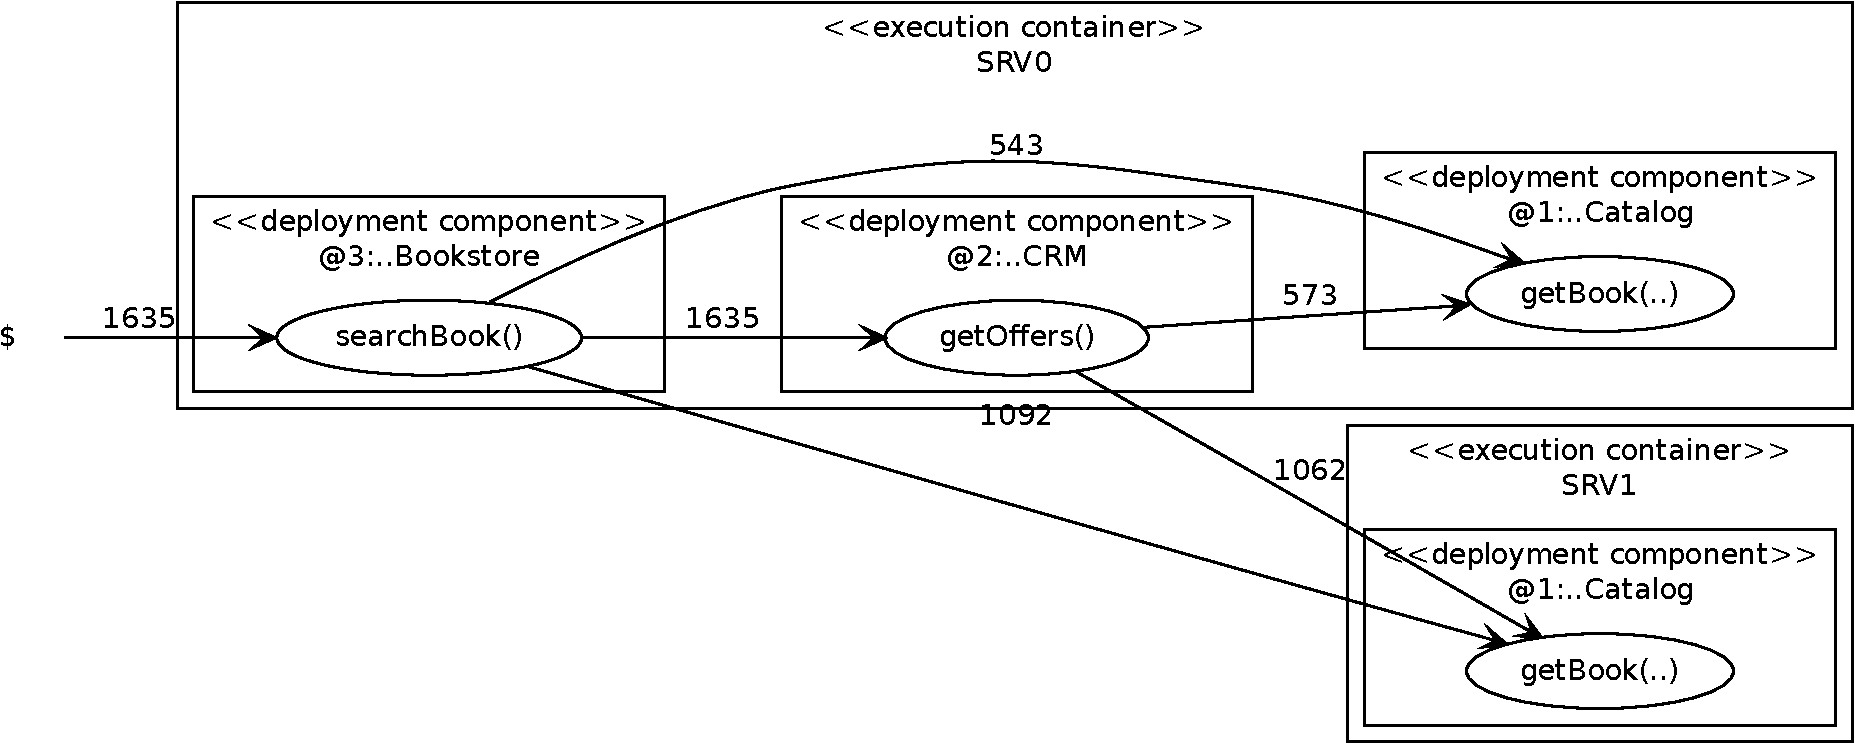
\includegraphics[scale=0.4]{../../examples/userguide/ch5--trace-monitoring-aspectj/testdata/kieker-20100830-082225522-UTC-example-plots/deploymentOperationDependencyGraph-crop}
}
\subfigure[assembly-level]{\label{fig:appendix:traceAnalysisExample:OperationDepGraphsAssembly}%
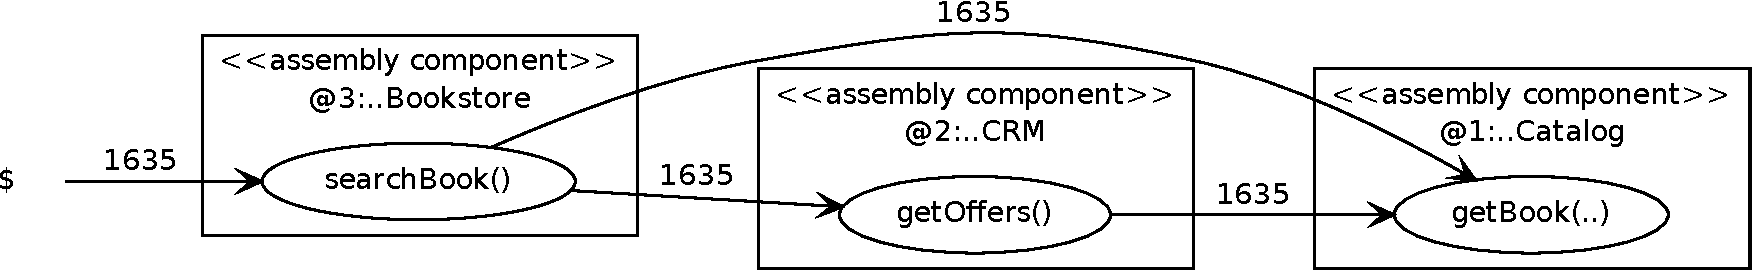
\includegraphics[scale=0.4]{../../examples/userguide/ch5--trace-monitoring-aspectj/testdata/kieker-20100830-082225522-UTC-example-plots/assemblyOperationDependencyGraph-crop}
}
\caption{Operation dependency graphs}
\label{fig:appendix:traceAnalysisExample:OperationDepGraphs}
\end{figure}

\pagebreak

\subsection{Response Times in Dependency Graphs}

The afore-mentioned dependency graphs can also be decorated by the response times, adding the minimum, the average, %
and the maximum response times of the components. The decoration will be generated with the additional command line %
parameter \OPT{responseTimes} behind the corresponding \OPT{plot-}command.  %
An exemplaric graph with response times is shown in Figure~\ref{fig:appendix:traceAnalysisExample:graphWithRespTimes}.

\begin{figure}[h]
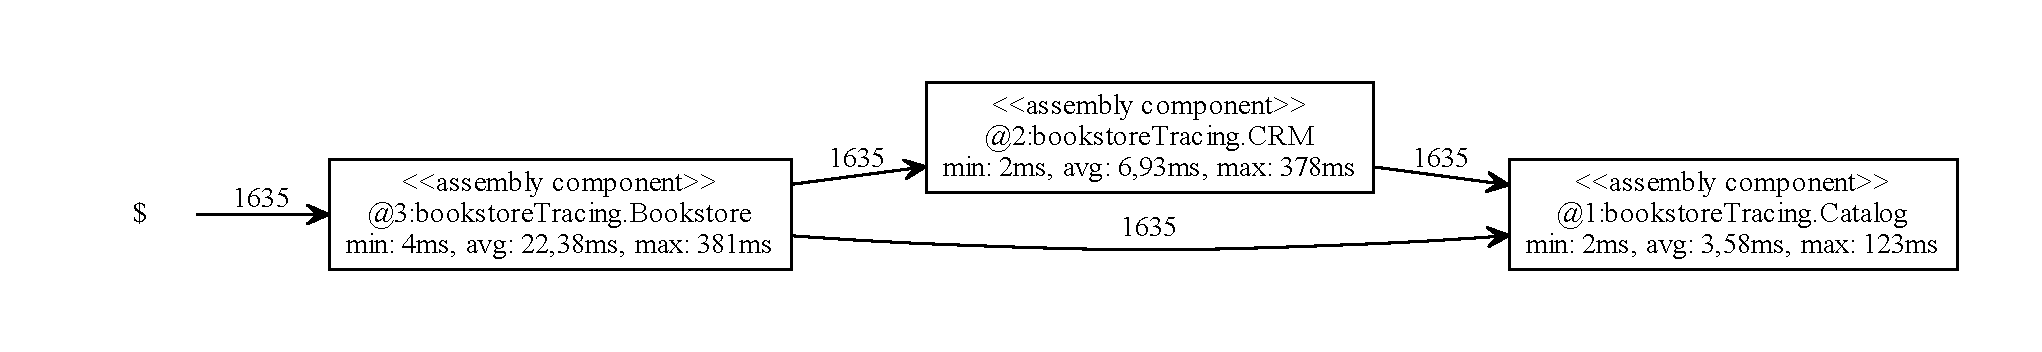
\includegraphics[scale=0.45]{images/assemblyComponentDependencyGraphWithResponseTimes}
\caption{Assembly component dependency graph with response times}
\label{fig:appendix:traceAnalysisExample:graphWithRespTimes}
\end{figure}
   

\pagebreak

\subsection{HTML Output of the System Model}

\KiekerTraceAnalysis{} writes an HTML representation of the system model reconstructed %
from the trace data to a file \file{system-entities.html}. %
Figure~\ref{fig:appendix:traceAnalysisExample:htmlSystemModel} shows a screenshot %
of this file rendered by a web browser.

\begin{figure}[h]\centering
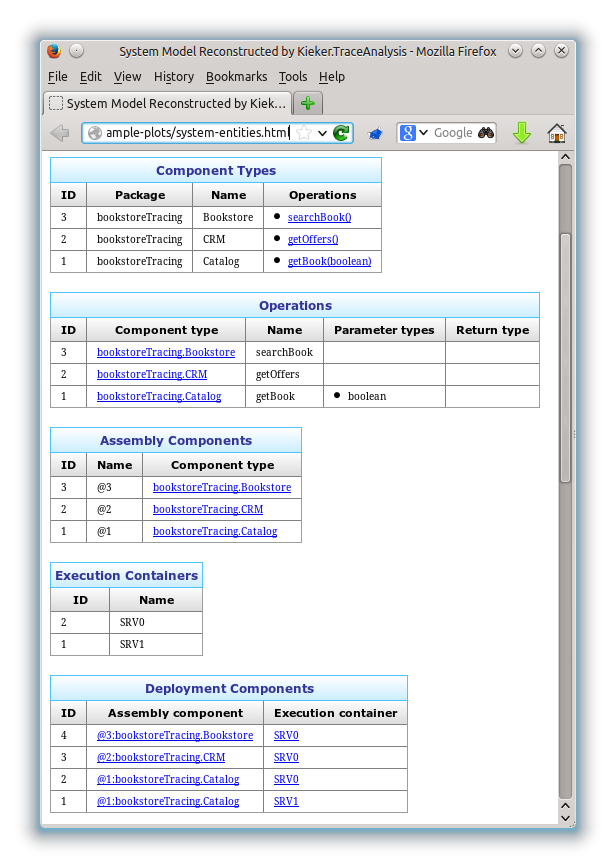
\includegraphics[width=0.7\textwidth]{images/system-entities-html-FFscrsh.png}
\caption{HTML output of the system model reconstructed from the traces}
\label{fig:appendix:traceAnalysisExample:htmlSystemModel}
\end{figure}



  %%%%%%%%%%%%%%%%%%%%%%%%%%%%%%%%%%%%%%%%%
% Appendix
% 
% $Date$
% $Rev$:
% $Author$


\appendix
\renewcommand{\thesection}{\Alph{section}} \setcounter{section}{0}
\chapter*{Appendix}
\addcontentsline{toc}{chapter}{Appendix}
  \section{\KiekerMonitoringPart{} Configuration File}\label{sec:appdx:monitoringproperties}

This is the file \file{\monitoringPropertiesFile} from the binary release and 
constitutes \KiekerMonitoringPart{}'s default configuration.

\

\setXMLListing
\lstinputlisting[caption=\monitoringPropertiesFile]{../../META-INF/kieker.monitoring.properties}

\newpage


  \section{Additional Source Code Listings}
    \subsection{MyNamedPipeManager and MyPipe}
      \setJavaCodeListing
      \lstinputlisting[caption=MyNamedPipeManager.java]{\customComponentsBookstoreApplicationDir/src/bookstoreTracing/MyNamedPipeManager.java}

      \setJavaCodeListing
      \lstinputlisting[caption=MyPipe.java]{\customComponentsBookstoreApplicationDir/src/bookstoreTracing/MyPipe.java}

\newpage
  \section{Example File System Monitoring Logs}

	\subsection{Chapter \ref{chap:example}}
		The following listing shows the produced log during a run of the Bookstore Application with the manual monitoring probes.
		\setTextListing
\begin{lstlisting}[caption=Execution of the manually instrumented Bookstore application (Section~\ref{sec:example:monitoring})]
Apr 28, 2011 5:15:25 PM kieker.monitoring.core.configuration.Configuration createSingletonConfiguration
INFO: Loading properties from properties file in classpath: 'META-INF/kieker.monitoring.properties'
Apr 28, 2011 5:15:25 PM kieker.monitoring.core.configuration.Configuration loadConfigurationFromResource
WARNING: File 'META-INF/kieker.monitoring.properties' not found in classpath
Apr 28, 2011 5:15:25 PM kieker.monitoring.core.controller.MonitoringController createInstance
INFO: Current State of kieker.monitoring (1.3-20110427) Status: 'enabled'
	Name: 'KIEKER-SINGLETON'; Hostname: 'Kaapstad'; experimentID: '1'
WriterController:
	Number of Inserts: '0'
	Automatic assignment of logging timestamps: 'true'
Writer: 'kieker.monitoring.writer.filesystem.AsyncFsWriter'
	Configuration:
		kieker.monitoring.writer.filesystem.AsyncFsWriter.QueueFullBehavior='0'
		kieker.monitoring.writer.filesystem.AsyncFsWriter.QueueSize='10000'
		kieker.monitoring.writer.filesystem.AsyncFsWriter.customStoragePath=''
		kieker.monitoring.writer.filesystem.AsyncFsWriter.storeInJavaIoTmpdir='true'
	Writer Threads (1): 
		Finished: 'false'; Writing to Directory: '/tmp/kieker-20110428-151525684-UTC-Kaapstad-KIEKER-SINGLETON'
Sampling Controller: Periodic Sensor available: Current Poolsize: '0'; Scheduled Tasks: '0'
Bookstore.main: Starting request 0
Bookstore.main: Starting request 1
Apr 28, 2011 5:15:25 PM kieker.monitoring.writer.filesystem.MappingFileWriter writeMapping
INFO: Registered monitoring record type with id '1':kieker.common.record.OperationExecutionRecord
Bookstore.main: Starting request 2
Bookstore.main: Starting request 3
Bookstore.main: Starting request 4
\end{lstlisting}

		The second listing is the log during the analysis of the produced data. It can be seen that some of the calls are accepted and some others refused.
		\setTextListing
\begin{lstlisting}[caption=Execution of the example analysis (Section~\ref{sec:example:analysis})]
19.08.2010 13:19:55 kieker.analysis.AnalysisController registerPlugin
INFO: Registered plugin bookstoreApplication.Consumer@6ac2a132
19.08.2010 13:19:55 kieker.analysis.AnalysisController registerPlugin
INFO: Plugin bookstoreApplication.Consumer@6ac2a132 also registered as record consumer
19.08.2010 13:19:55 kieker.analysis.reader.filesystem.FSDirectoryReader processInputFile
INFO: < Loading C:\Temp\tpmon-20100814-103954167-UTC\tpmon-20100814-103954184-UTC-Thread-2.dat
19.08.2010 13:19:55 kieker.common.record.MonitoringRecordTypeRegistry registerRecordTypeIdMapping
INFO: Registered record type mapping 1/kieker.common.record.OperationExecutionRecord
maximal response time exceeded by 11382559 ns: bookstoreApplication.Catalog.getBook()
maximal response time exceeded by 11251720 ns: bookstoreApplication.Catalog.getBook()
maximal response time exceeded by 80320 ns: bookstoreApplication.Catalog.getBook()
maximal response time exceeded by 27400 ns: bookstoreApplication.Catalog.getBook()
maximal response time exceeded by 81760 ns: bookstoreApplication.Catalog.getBook()
maximal response time exceeded by 24240 ns: bookstoreApplication.Catalog.getBook()
maximal response time exceeded by 82480 ns: bookstoreApplication.Catalog.getBook()
response time accepted: bookstoreApplication.Catalog.getBook()
response time accepted: bookstoreApplication.Catalog.getBook()
response time accepted: bookstoreApplication.Catalog.getBook()
14.08.2010 12:41:02 kieker.analysis.reader.filesystem.FSReader$\$$FSReaderCons execute
INFO: All reader threads provided FS_READER_TERMINATION_MARKER
\end{lstlisting}
	
	\subsection{Chapter \ref{chap:aspectJ}}
	    The following listing shows the produced log during a run of the Bookstore Application, weaved with the necessary code at runtime as shown in Section \ref{sec:aspectJ:fullweaving}.
		\setTextListing
\begin{lstlisting}[caption=Execution of the Bookstore with AspectJ trace instrumentation (Section~\ref{sec:traceAnalysis:instr:AspectJ})]
Bookstore.main: Starting request 0
Apr 28, 2011 4:28:29 PM kieker.monitoring.core.configuration.Configuration createSingletonConfiguration
INFO: Loading properties from properties file in classpath: 'META-INF/kieker.monitoring.properties'
Apr 28, 2011 4:28:29 PM kieker.monitoring.core.controller.MonitoringController createInstance
INFO: Current State of kieker.monitoring (1.3-20110427) Status: 'enabled'
	Name: 'KIEKER'; Hostname: 'Kaapstad'; experimentID: '1'
WriterController:
	Number of Inserts: '0'
	Automatic assignment of logging timestamps: 'true'
Writer: 'kieker.monitoring.writer.filesystem.AsyncFsWriter'
	Configuration:
		kieker.monitoring.writer.filesystem.AsyncFsWriter.QueueFullBehavior='0'
		kieker.monitoring.writer.filesystem.AsyncFsWriter.QueueSize='10000'
		kieker.monitoring.writer.filesystem.AsyncFsWriter.customStoragePath=''
		kieker.monitoring.writer.filesystem.AsyncFsWriter.storeInJavaIoTmpdir='true'
	Writer Threads (1): 
		Finished: 'false'; Writing to Directory: '/tmp/kieker-20110428-142829399-UTC-Kaapstad-KIEKER'
Sampling Controller: Periodic Sensor available: Current Poolsize: '0'; Scheduled Tasks: '0'
Apr 28, 2011 4:28:29 PM kieker.monitoring.core.registry.ControlFlowRegistry <init>
INFO: First threadId will be 7752665283541598209
Apr 28, 2011 4:28:29 PM kieker.monitoring.writer.filesystem.MappingFileWriter writeMapping
INFO: Registered monitoring record type with id '1':kieker.common.record.OperationExecutionRecord
\end{lstlisting}



	
\newpage
  \section{Ant Scripts}
    \subsection{Chapter \ref{chap:example}}
      Following listings show the necessary \file{build.xml} and \file{build.properties} to compile and execute the manual instrumentated Bookstore Application shown in Chapter~\ref{chap:example}.
      \setXMLListing
      \lstinputlisting[caption=build.xml]{\manualInstrumentedBookstoreApplicationDir/build.xml}
      \lstinputlisting[caption=build.properties]{\manualInstrumentedBookstoreApplicationDir/build.properties}
      In order to run the analysis of the application, it is still necessary to supply the program with the path to the output directory of the monitoring. This is done via the parameter "analysis.directory", e.g.:
      \setBashListing
      \begin{lstlisting}[caption=Command to compile and run the instrumented Bookstore via ant]
#\lstshellprompt{}# ant run-analysis -Danalysis.directory /tmp/kicker-20120402-163314855-UTC-myHost-KIEKER-SINGLETON
\end{lstlisting}%-KIEKER


    \subsection{Chapter \ref{chap:componentsMonitoring} and \ref{chap:componentsAnalysis}}
      Following listings show the necessary \file{build.xml} and \file{build.properties} to compile and execute the manually instrumentated Bookstore Application with the own components shown in Chapter~\ref{chap:componentsMonitoring} and \ref{chap:componentsAnalysis}.
      \setXMLListing
      \lstinputlisting[caption=build.xml]{\customComponentsBookstoreApplicationDir/build.xml}
      \lstinputlisting[caption=build.properties]{\customComponentsBookstoreApplicationDir/build.properties}

    \subsection{Chapter \ref{chap:aspectJ}}
      Following listings show the necessary \file{build.xml} and \file{build.properties} to compile and execute the Bookstore Application instrumentated with AspectJ shown in Chapter~\ref{chap:aspectJ}.
      \setXMLListing
      \lstinputlisting[caption=build.xml]{\aspectJBookstoreApplicationDir/build.xml}
      \lstinputlisting[caption=build.properties]{\aspectJBookstoreApplicationDir/build.properties}     

\newpage
  \section{Example Graphs and Diagrams}
    \begin{figure}[H]\centering
	\subfigure[]{\label{fig:appendix:aggregatedAllocationCallTree}%
	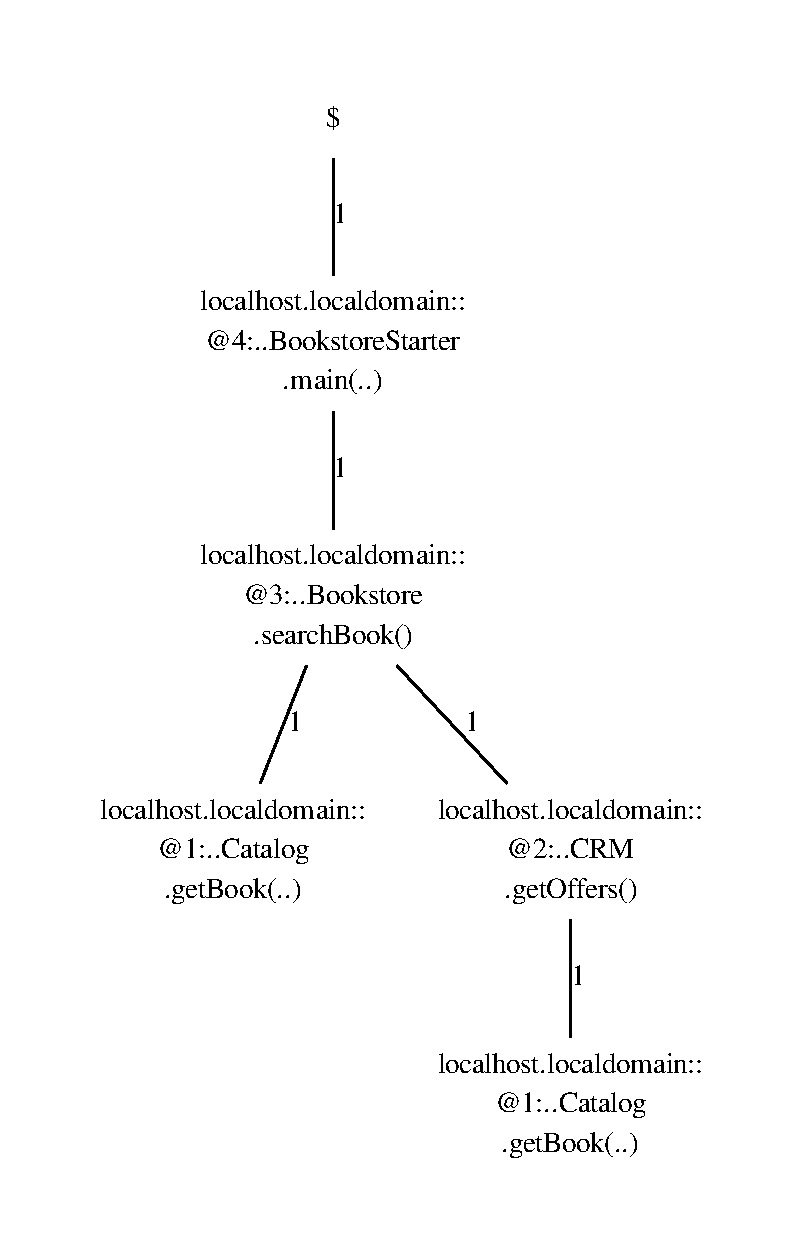
\includegraphics[width=0.33\textwidth]{images/aggregatedAllocationCallTree}%
	}%
	\subfigure[]{\label{fig:appendix:aggregatedAssemblyCallTree}%
	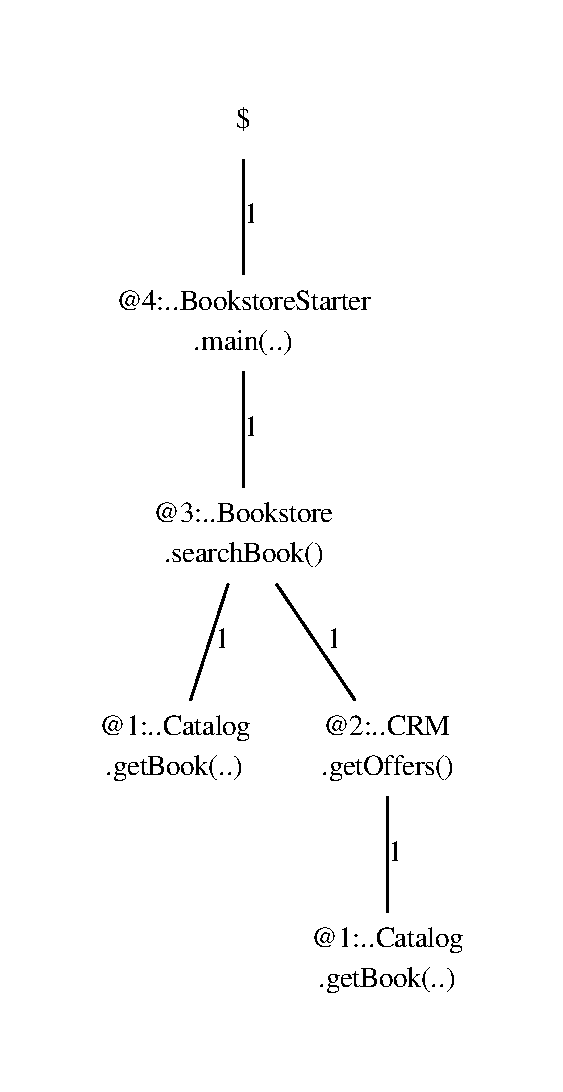
\includegraphics[width=0.33\textwidth]{images/aggregatedAssemblyCallTree}%
	}%
	\subfigure[]{\label{fig:appendix:callTree}%
	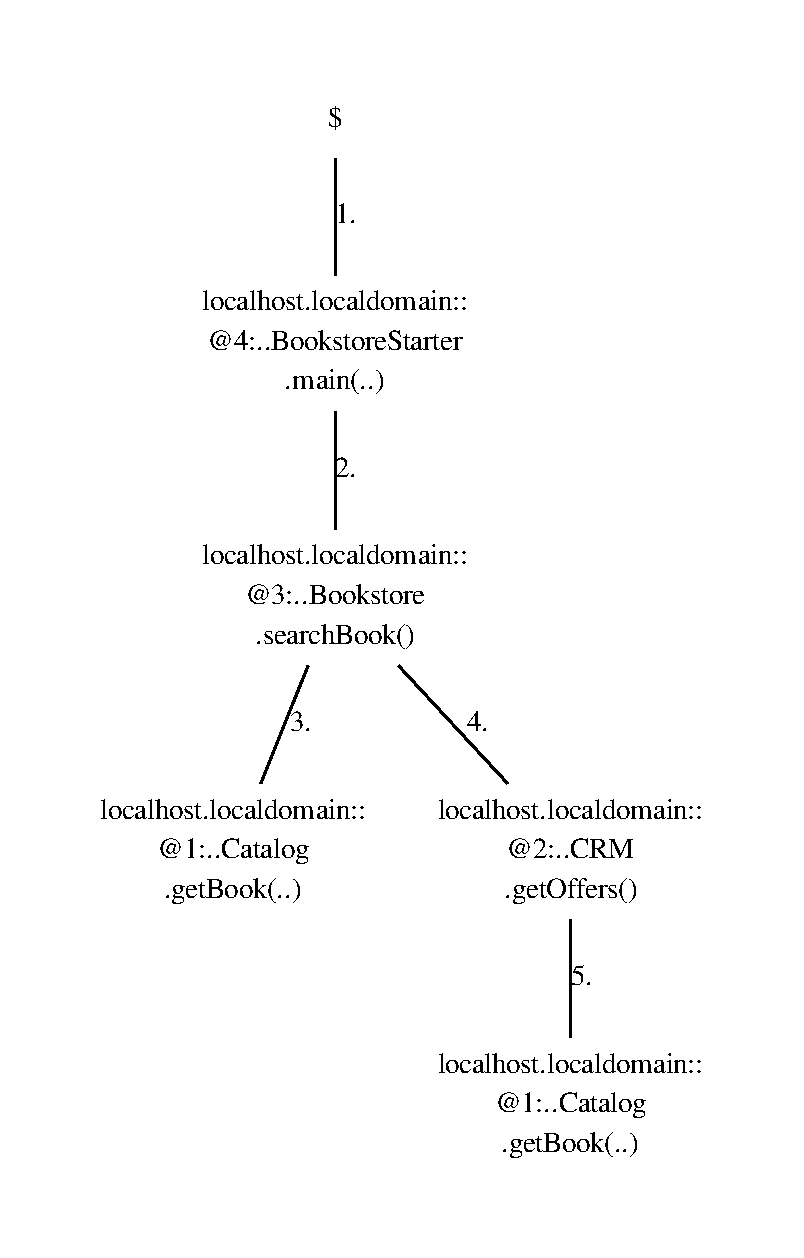
\includegraphics[width=0.33\textwidth]{images/callTree}%
	}%
	\caption{Aggregated Allocation Call Tree~\subref{fig:appendix:aggregatedAllocationCallTree}, Aggregated Assembly Call Tree~\subref{fig:appendix:aggregatedAssemblyCallTree} and Call Tree~\subref{fig:appendix:callTree}}
	\end{figure}
	
    \begin{figure}[H]\centering
	\subfigure[]{\label{fig:appendix:allocationComponentDependencyGraph}%
	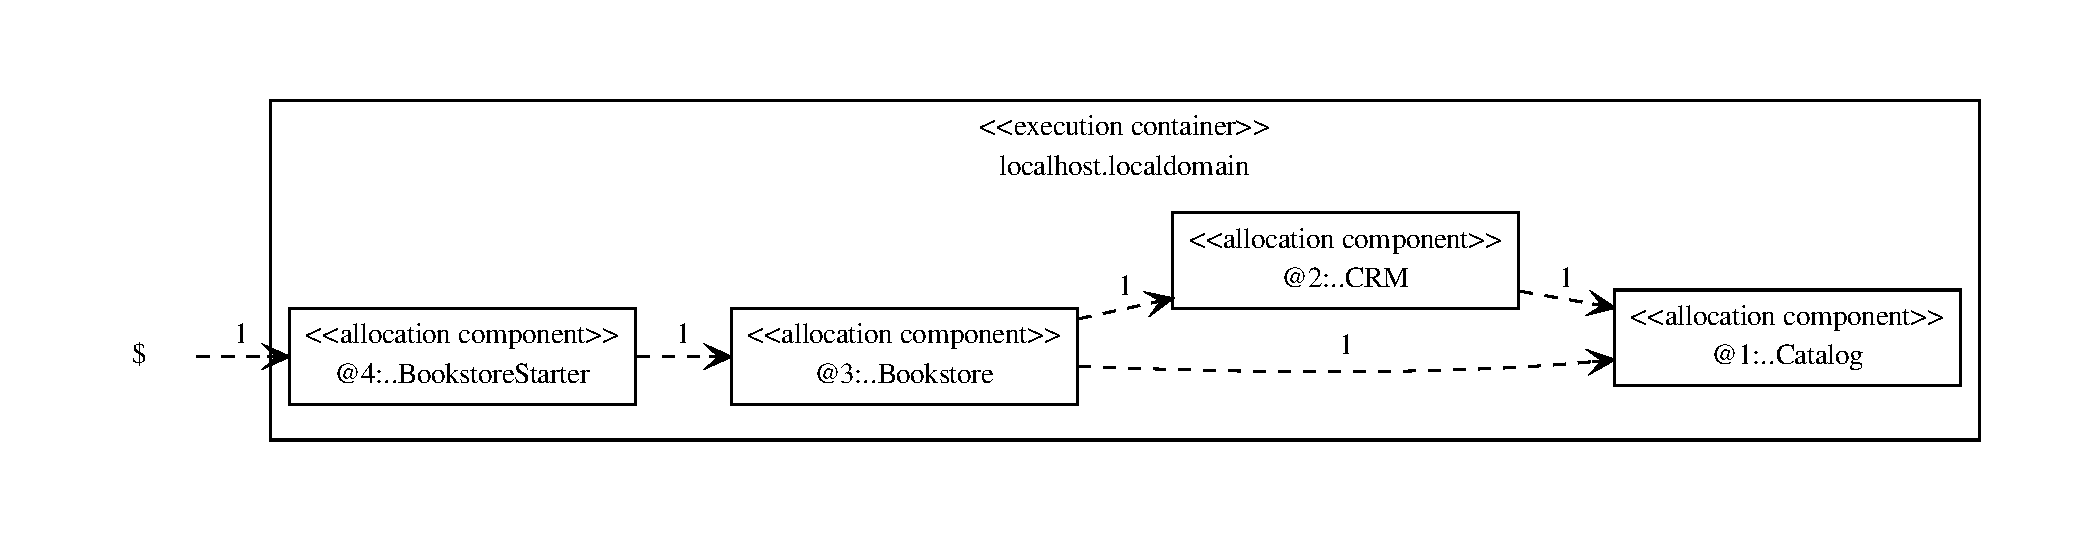
\includegraphics[width=0.8\textwidth]{images/allocationComponentDependencyGraph}
	}\\
	\subfigure[]{\label{fig:appendix:assemblyComponentDependencyGraph}%
	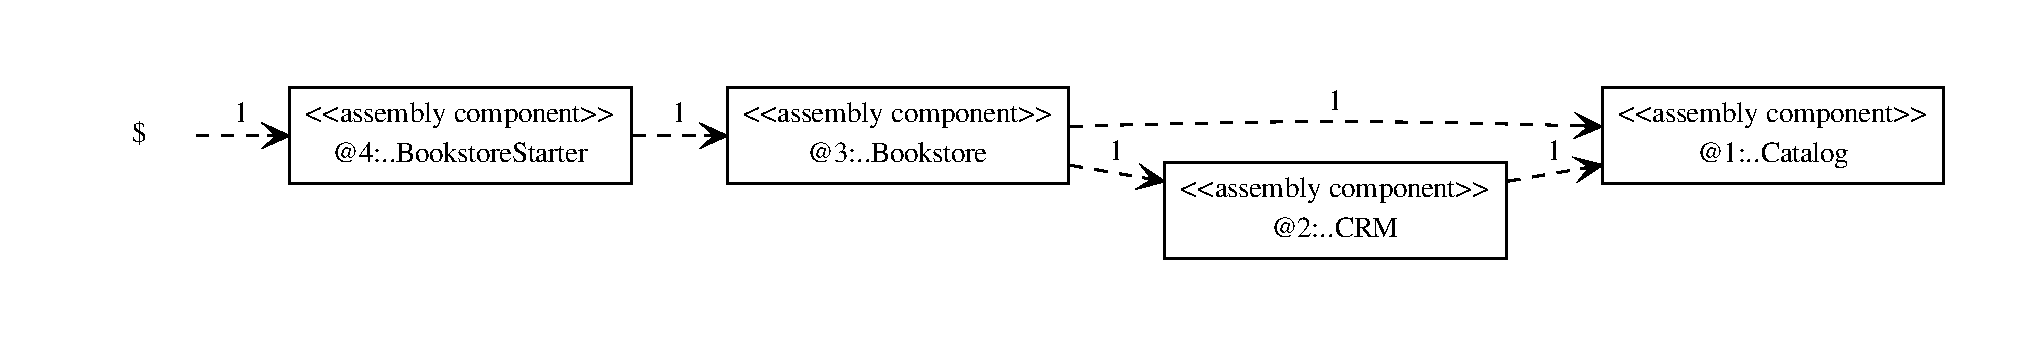
\includegraphics[width=0.8\textwidth]{images/assemblyComponentDependencyGraph}
	}%
	\caption{Allocation Component Dependency Graph~\subref{fig:appendix:allocationComponentDependencyGraph} and Assembly Component Dependency Graph~\subref{fig:appendix:assemblyComponentDependencyGraph}}
	\end{figure}
	
	\begin{figure}[H]\centering
	\subfigure[]{\label{fig:appendix:allocationOperationDependencyGraph}%
	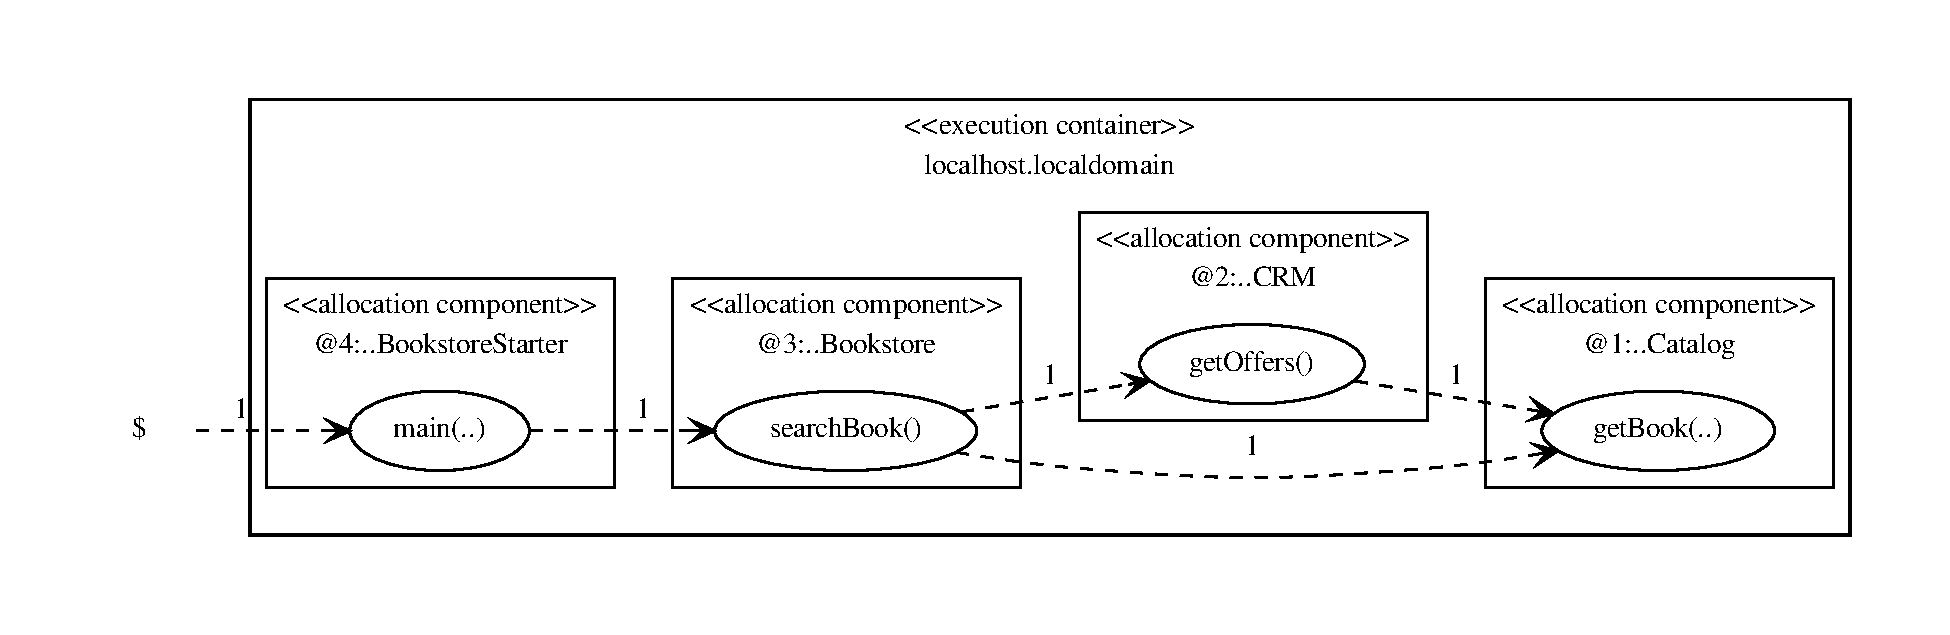
\includegraphics[width=0.8\textwidth]{images/allocationOperationDependencyGraph}
	}\\
	\subfigure[]{\label{fig:appendix:assemblyOperationDependencyGraph}%
	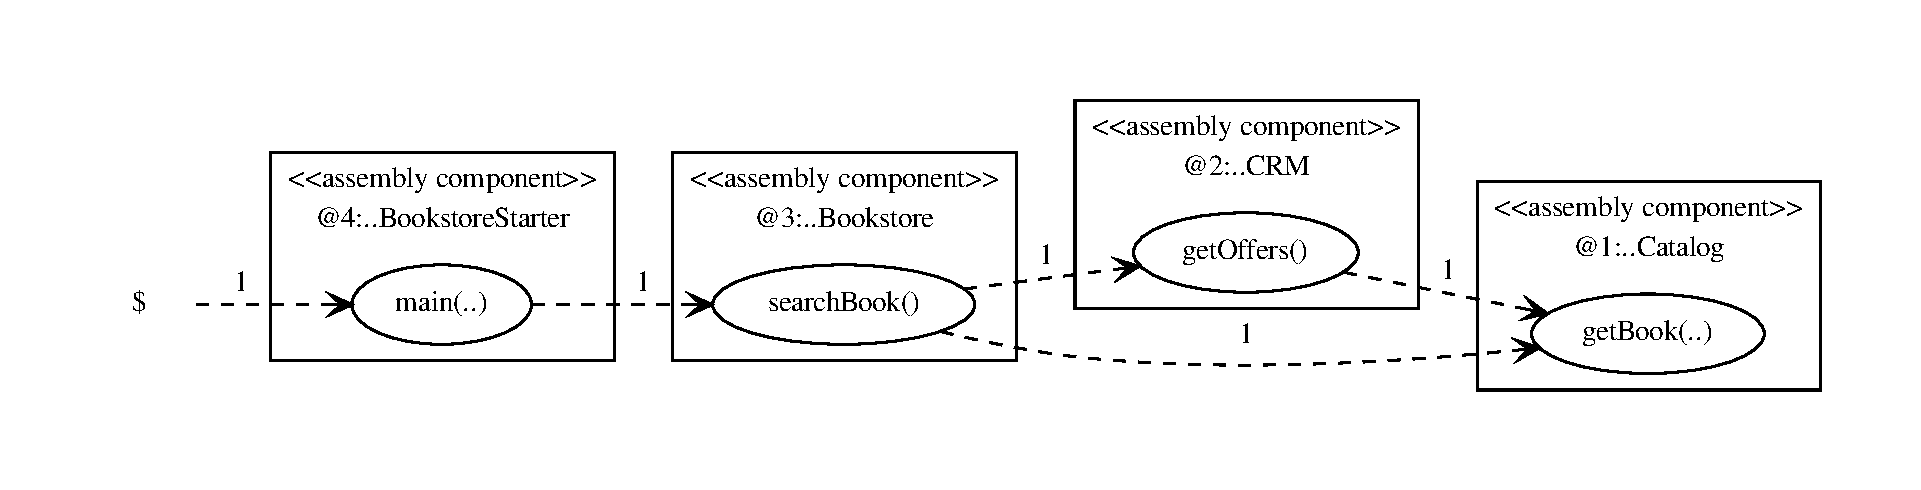
\includegraphics[width=0.8\textwidth]{images/assemblyOperationDependencyGraph}
	}%
	\caption{Allocation Operation Dependency Graph~\subref{fig:appendix:allocationOperationDependencyGraph} and Allocation Operation Dependency Graph~\subref{fig:appendix:assemblyOperationDependencyGraph}}
	\end{figure}
	
	\begin{figure}[H]\centering
	\subfigure[]{\label{fig:appendix:allocationSequenceDiagram}
	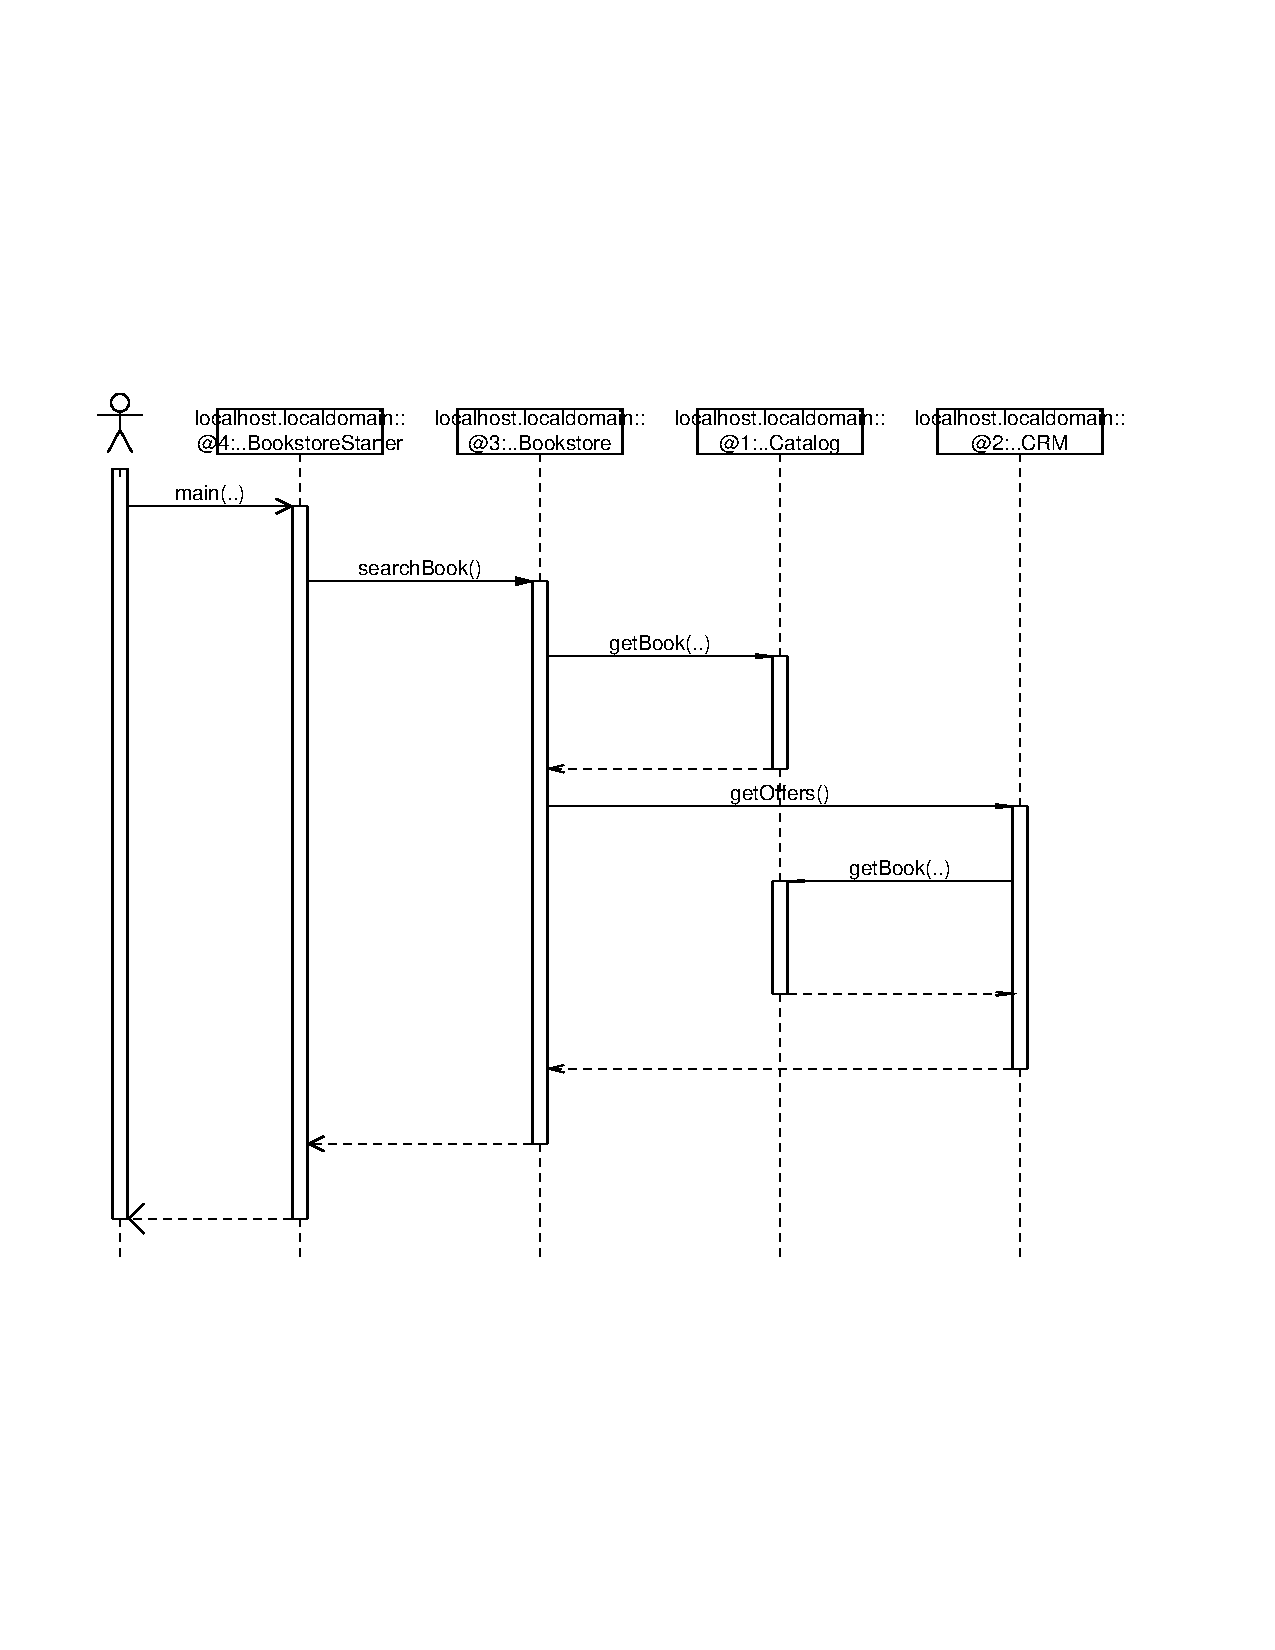
\includegraphics[width=0.4\textwidth]{images/allocationSequenceDiagram}
	}
	\subfigure[]{\label{fig:appendix:assemblySequenceDiagram}
	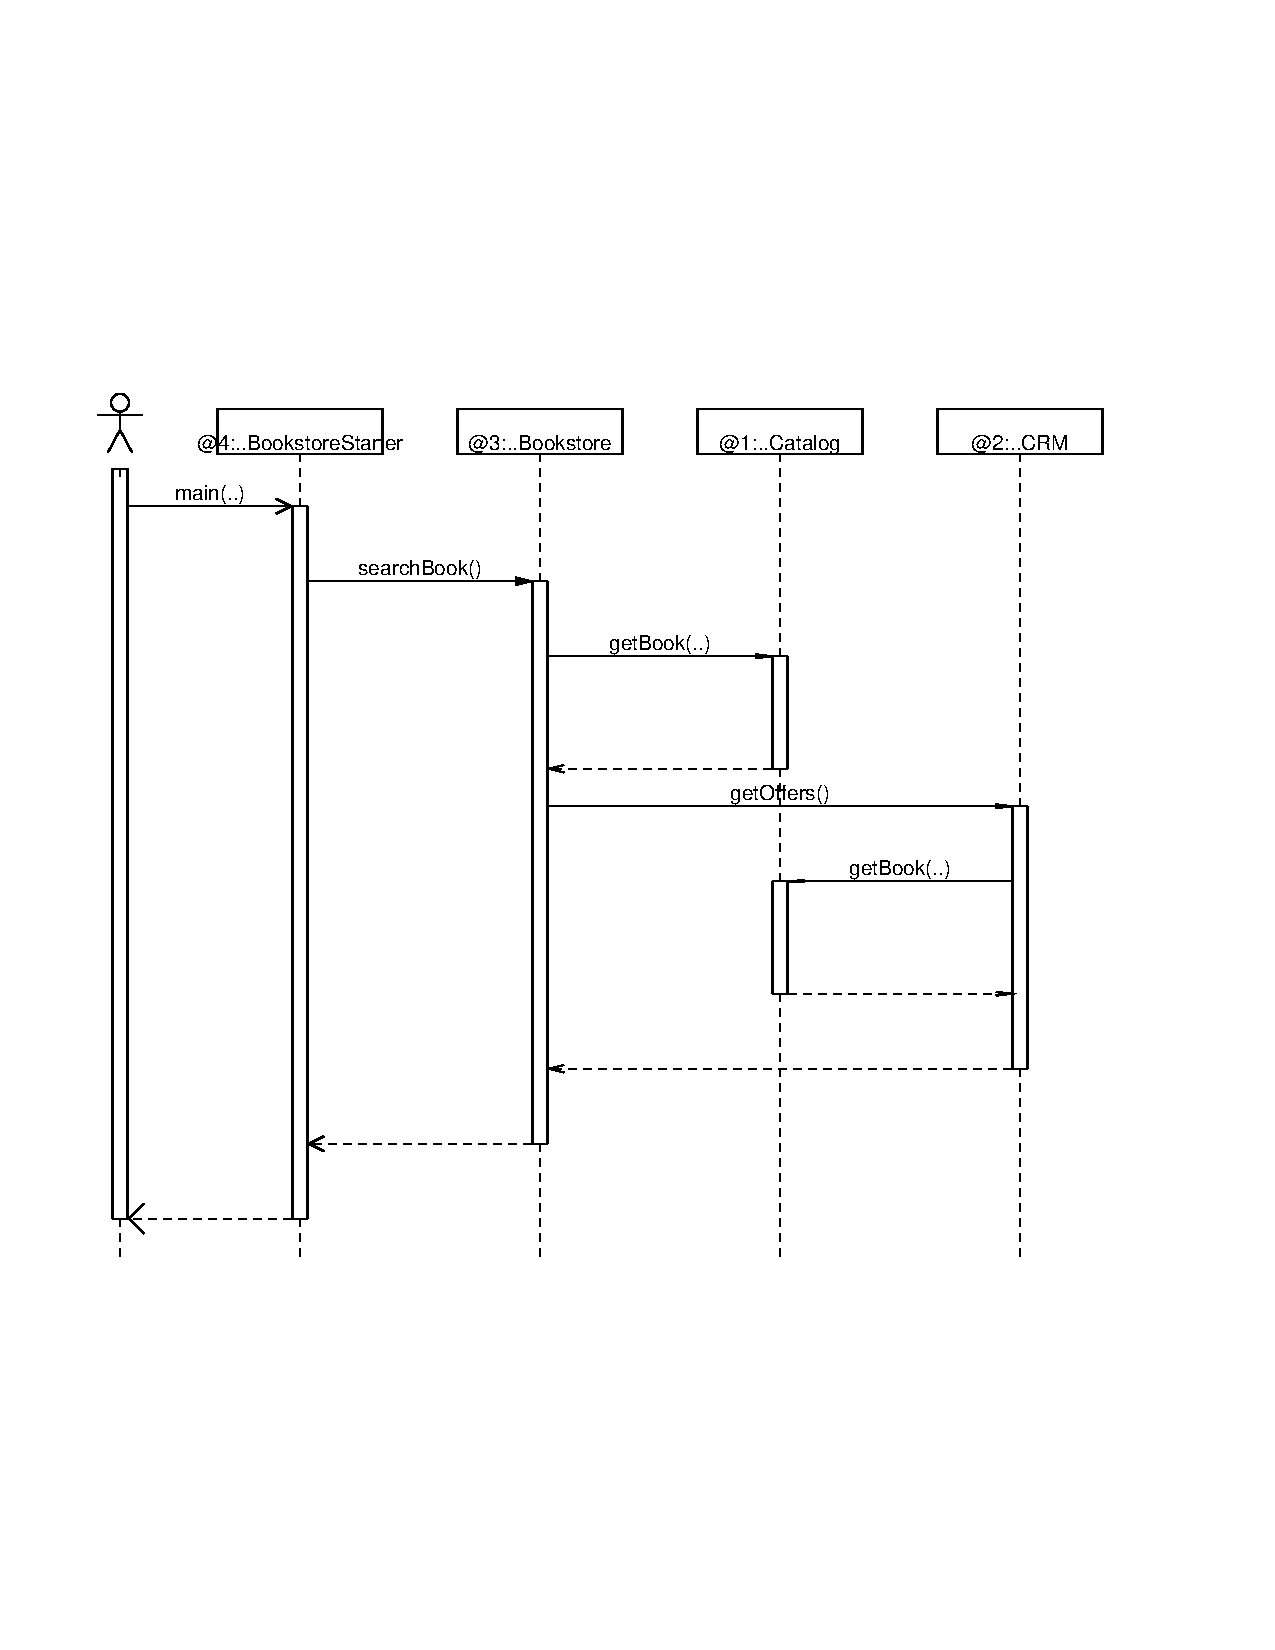
\includegraphics[width=0.4\textwidth]{images/assemblySequenceDiagram}
	}
	\caption{Allocation Sequence Diagram~\subref{fig:appendix:allocationSequenceDiagram} and Assembly Sequence Diagram~\subref{fig:appendix:assemblySequenceDiagram}}
	\end{figure}
	
	\begin{figure}[H]
		\centering
		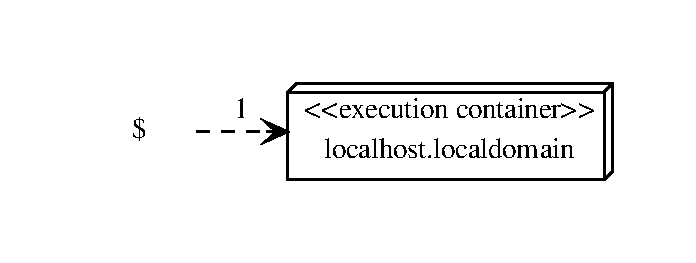
\includegraphics[width=0.5\textwidth]{images/containerDependencyGraph}
		\caption{Container Dependency Graph}
	\end{figure}
  
  
\newpage
  \section{Libraries}
    The following table shows all libraries which are used by \Kieker\ and explains them briefly.
    \begin{center}
\begin{longtable}{|p{0.4\textwidth}|p{0.5\textwidth}|}
\hline 
Filename & Description\\
\hline
\hline 
commons-cli-1.2.jar & n/a\\
\hline 
maven & n/a\\
\hline 
mysql-connector-java-5.1.5-bin.jar & The library to connect to an existing MySQL database.\\
\hline 
spring-web.jar & n/a\\
\hline 
Scenario.jar & n/a\\
\hline 
sequence.pic & n/a\\
\hline 
openjms-0.7.7-beta-1.tar.gz & n/a\\
\hline 
aspectjrt-1.6.6.jar & n/a\\
\hline 
commons-logging-1.1.1.jar & n/a\\
\hline 
aspectjtools-1.6.6.jar & n/a\\
\hline 
jms-1.1.jar & n/a\\
\hline 
concurrent-1.3.4.jar & n/a\\
\hline 
servlet.jar & n/a\\
\hline 
pmd & n/a\\
\hline 
spring.jar & n/a\\
\hline 
openjms-common-0.7.7-beta-1.jar & n/a\\
\hline 
servlet-api.jar & n/a\\
\hline 
commons-pool-1.2.jar & n/a\\
\hline 
derby.jar & This library contains the necessary drivers for the Apache Derby database.\\
\hline 
commons-io-1.2.jar & n/a\\
\hline 
cxf-rt-core-2.2.6.jar & n/a\\
\hline 
jmc.jar & n/a\\
\hline 
log4j-1.2.15.jar & n/a\\
\hline 
openjms-net-0.7.7-beta-1.jar & n/a\\
\hline 
aspectjweaver-1.6.6.jar & n/a\\
\hline 
cxf-api-2.2.6.jar & n/a\\
\hline 
rabbitmq-client.jar & n/a\\
\hline 
openjms-0.7.7-beta-1.jar & n/a\\
\hline 
spice-jndikit-1.2.jar & n/a\\
\hline 
cxf-rt-bindings-soap-2.2.6.jar & n/a\\
\hline 
cxf-common-utilities-2.2.6.jar & n/a\\
\hline 
jndi-1.2.1.jar & n/a\\
\hline 
\end{longtable}
\label{tabular:libraries}
\end{center}


% \chapter{Troubleshooting}

  % suppress appendix chapters in toc:
  \addtocontents{toc}{\protect\setcounter{tocdepth}{0}}

\bibliographystyle{abbrvnatAvanhoorn} % alpha
\bibliography{bibliography}
\end{document}

